
\chapter{Linear independence}

\index{linear independence}

One of the deepest and most central concepts in linear algebra -- in fact, if I
were to make a top ten ranking, this one might just make \#1 -- is that of
\textbf{linear independence}. It's not about mechanical computations, but
conceptual truths. Learn this chapter well. 

\section{The Domino Game}
\index{the Domino Game}

I've thought long and hard about the best way to teach the material in this
chapter, and I've come up with a game. I call it ``the Domino Game.'' Here are
the rules:

\begin{framed}
\begin{compactenum}
\item You are given one or more \textbf{yellow}\footnotemark ``starter dominoes.''
\item The object of the game is to build the white ``goal domino'' from these
starter dominoes.
\item You can ``use'' any number of each starter domino (even a fraction, even
negative), and add them together (left sides add together, and right sides add
together).
\item You \textit{cannot} use only one side of a domino.
\item You \textit{cannot} turn a domino around so the left side and right
sides flip.
\end{compactenum}
\end{framed}

\footnotetext{Light gray, actually, since I made this book black\&white to keep costs down.}

Example. Suppose your starter dominoes are:

\begin{center}
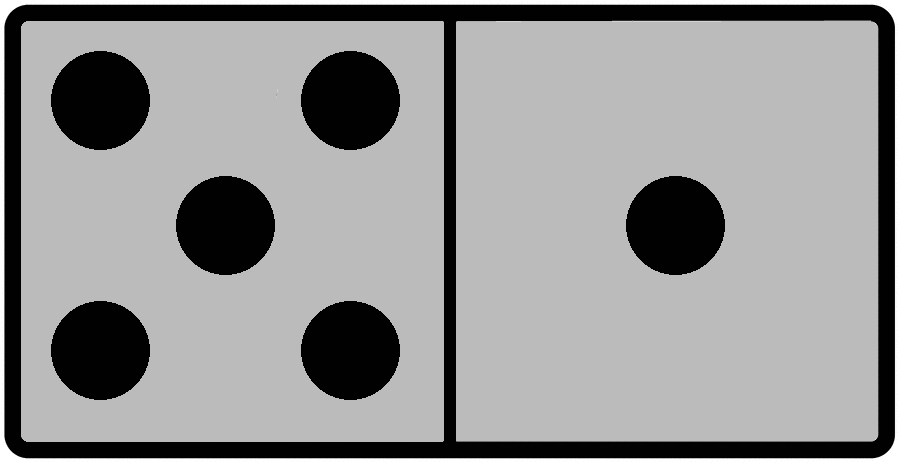
\includegraphics[width=0.3\textwidth]{gray5_1.png}
\hspace{.3in}
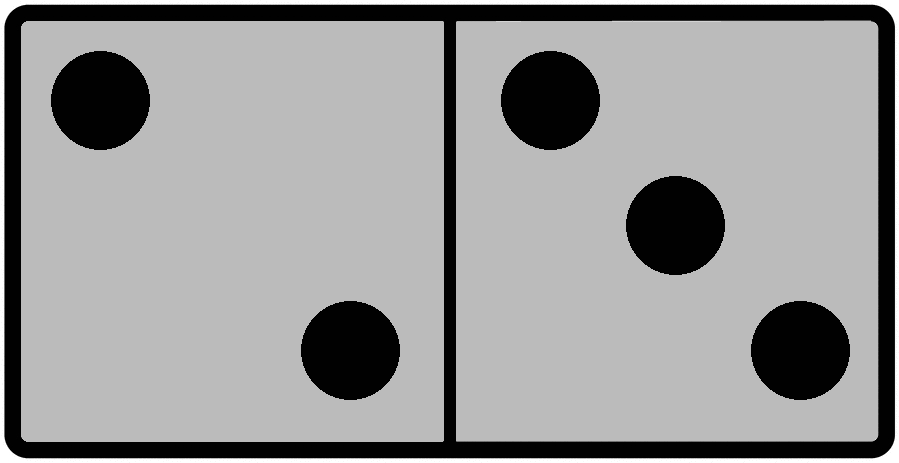
\includegraphics[width=0.3\textwidth]{gray2_3.png}
\end{center}

and your goal domino is:
\begin{center}
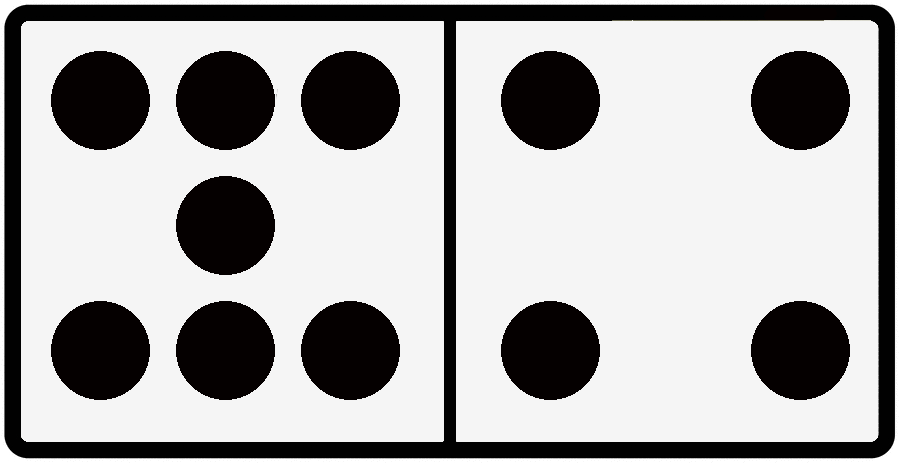
\includegraphics[width=0.3\textwidth]{white7_4.png}
\end{center}

A solution would be ``\textbf{one} and \textbf{one}.'' This means that you'll
take \textit{one} copy of the first starter domino, and \textit{one} copy of
the second, and add them together.

\begin{center}
{\LARGE Solution: \textbf{1 \& 1}}

1 \raisebox{-0.3\height}{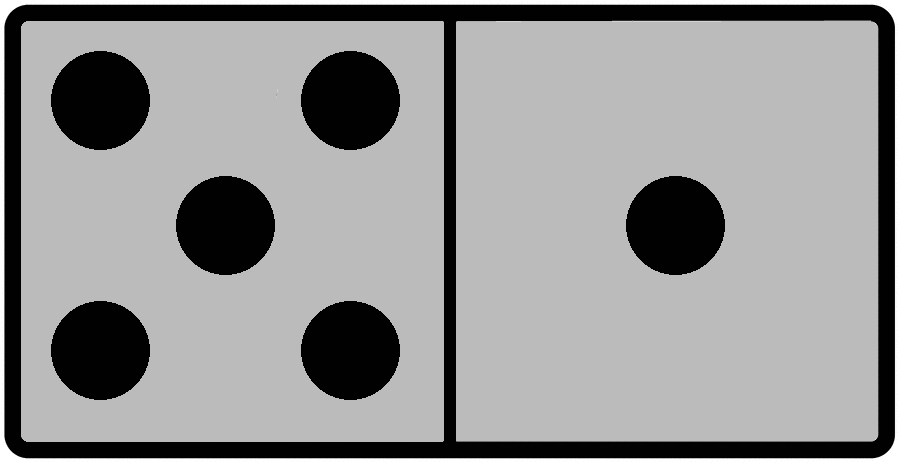
\includegraphics[width=0.1\textwidth]{gray5_1.png}} \ \& \
1 \raisebox{-0.3\height}{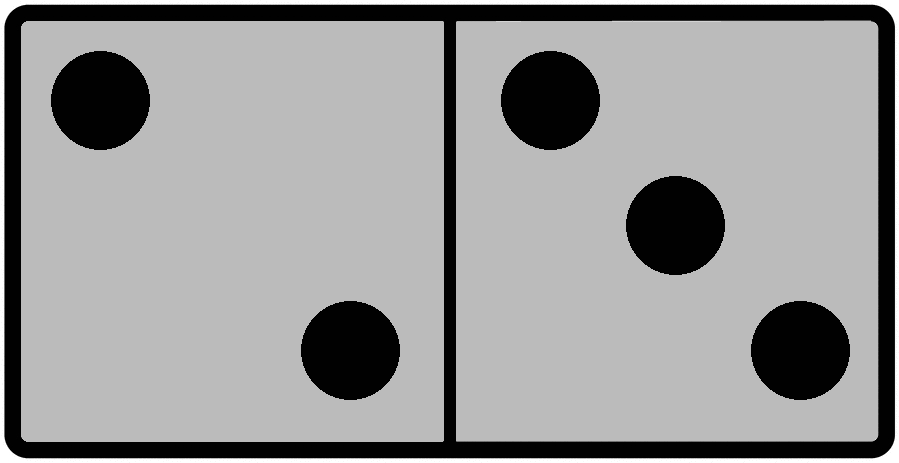
\includegraphics[width=0.1\textwidth]{gray2_3.png}} \ = \
\raisebox{-0.3\height}{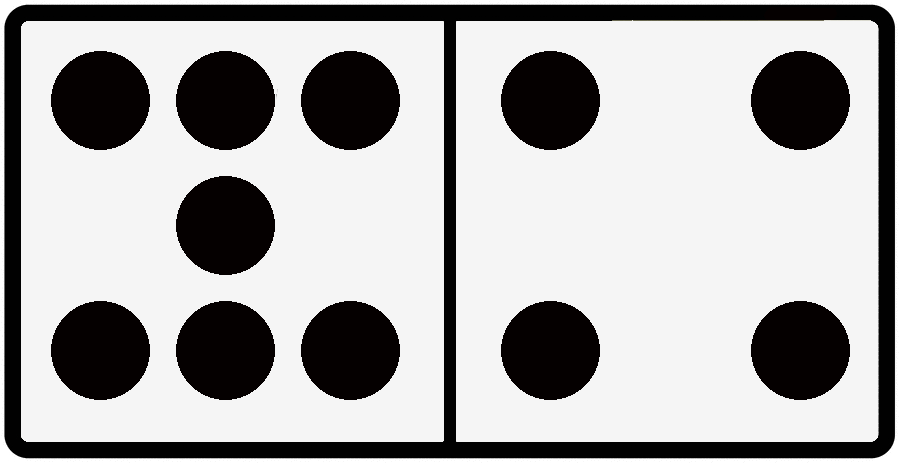
\includegraphics[width=0.1\textwidth]{white7_4.png}} \quad
\end{center}

Stare carefully at that until you master how it works; the rest of this chapter
will be a complete waste of time if this operation is not fully grasped. Adding
domino 5--1 to 2--3 means adding the left sides together, and separately adding
the right sides together, to produce a new domino 7--4 (since $5+2=7$ and
$1+3=4$).

\subsection{Actually do this}

All right, let's test your skillz. I want you to \textit{actually} work out the
answers to the following Domino Game puzzles on your own. There are six of
them, so it might take you a while (perhaps as long as 6 minutes). But it's
vital to cement your understanding of how this works...\textit{and} to set up
the crucial punchline later on in this chapter.

Answers to each puzzle are given at the end of the chapter. Maybe your answers
will not be the same as mine...or maybe they will? That itself is actually a
very important question we'll consider in a few minutes.

Enough preamble. Go!

\begin{enumerate}
\itemsep2em

\label{startDominoPuzzles}
\item Starter dominoes:
\hspace{.3in}
\raisebox{-0.3\height}{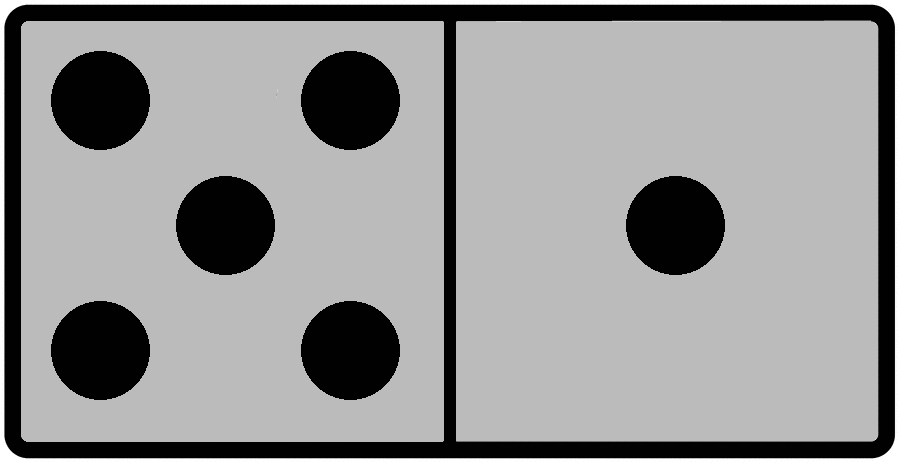
\includegraphics[width=0.2\textwidth]{gray5_1.png}}
\hspace{.1in}
\raisebox{-0.3\height}{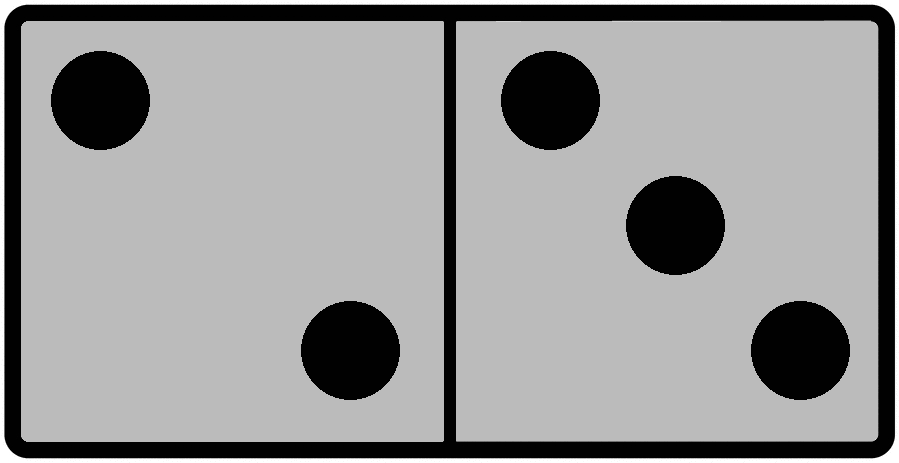
\includegraphics[width=0.2\textwidth]{gray2_3.png}}

Goal domino:
\hspace{1.1in}
\raisebox{-0.3\height}{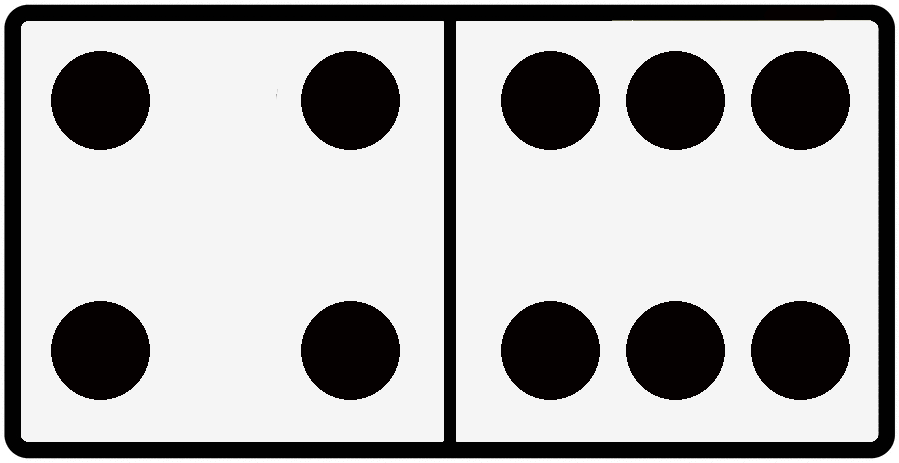
\includegraphics[width=0.2\textwidth]{white4_6.png}}

\footnotesize
(Hint: it's okay to take \textit{zero} of one of the dominoes; \textit{i.e.},
to completely ignore it.)
\normalsize

\item Starter dominoes:
\hspace{.3in}
\raisebox{-0.3\height}{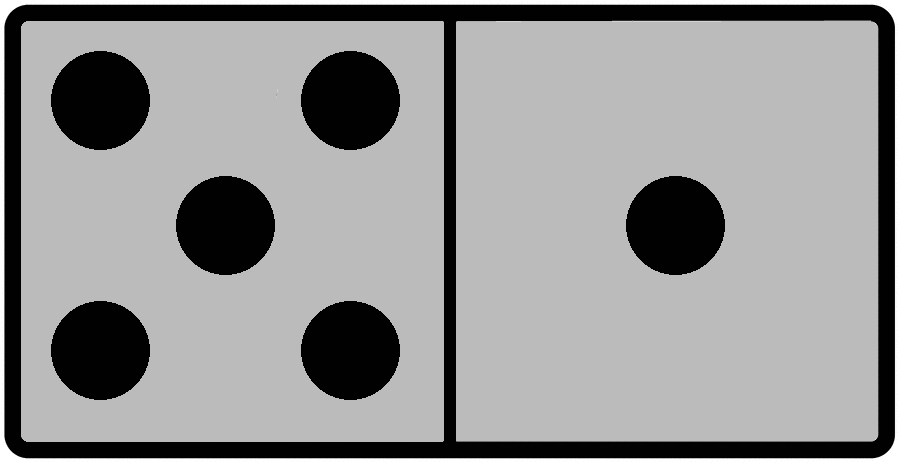
\includegraphics[width=0.2\textwidth]{gray5_1.png}}
\hspace{.1in}
\raisebox{-0.3\height}{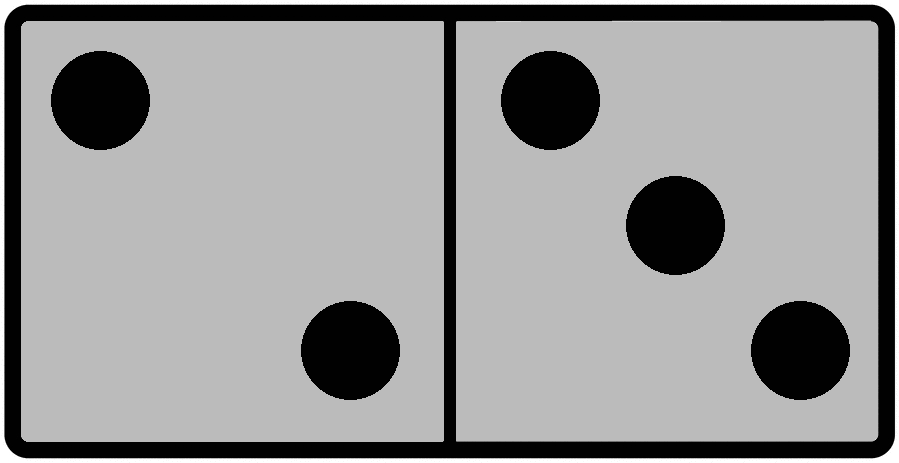
\includegraphics[width=0.2\textwidth]{gray2_3.png}}

Goal domino:
\hspace{1.1in}
\raisebox{-0.3\height}{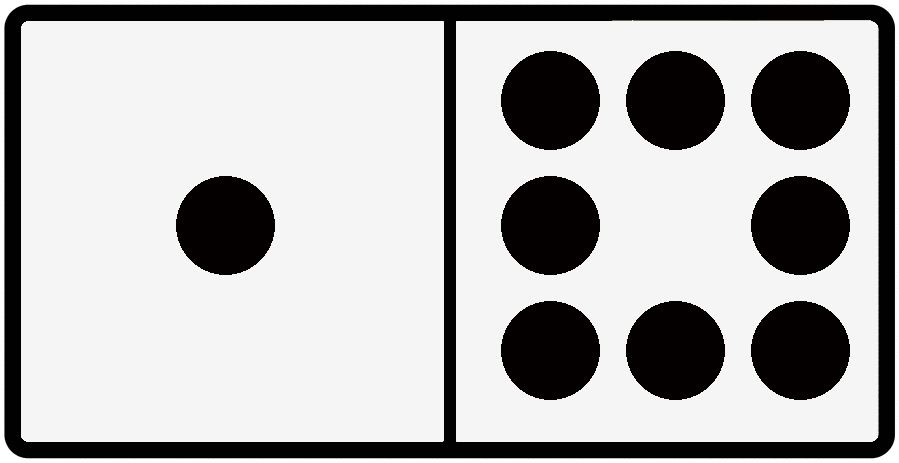
\includegraphics[width=0.2\textwidth]{white1_8.png}}

\footnotesize
(Hint: you may, if you wish, take ``a \textit{negative} number'' of one of the
dominoes. In other words, you can multiply the entire domino by a negative
number and then add it to your multiples of the other one.)
\normalsize

\item Starter dominoes:
\hspace{.3in}
\raisebox{-0.3\height}{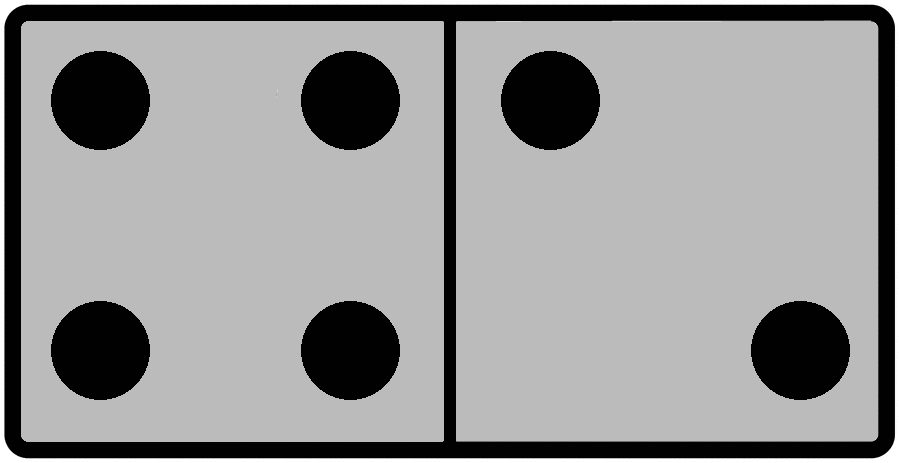
\includegraphics[width=0.2\textwidth]{gray4_2.png}}
\hspace{.1in}
\raisebox{-0.3\height}{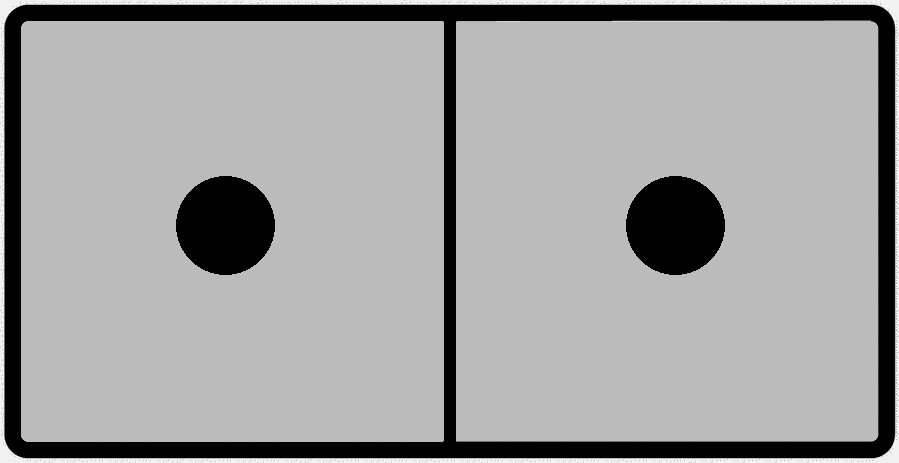
\includegraphics[width=0.2\textwidth]{gray1_1.png}}

Goal domino:
\hspace{1.1in}
\raisebox{-0.3\height}{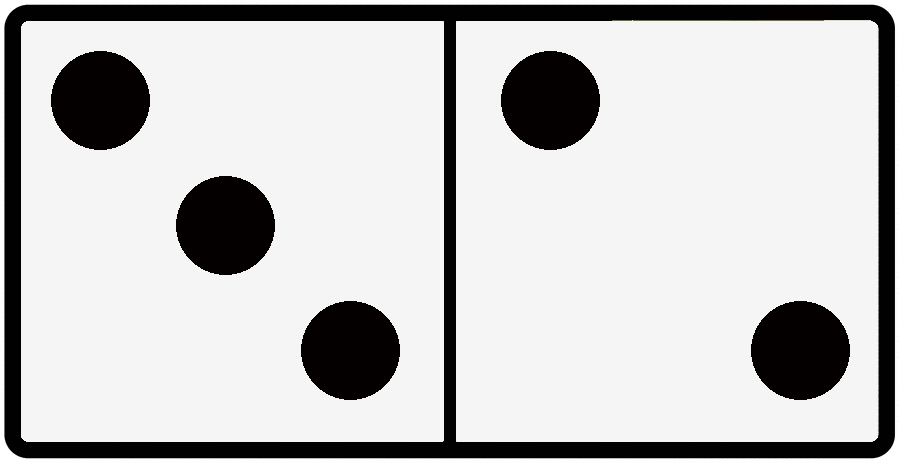
\includegraphics[width=0.2\textwidth]{white3_2.png}}

\footnotesize
(Hint: you can even take a \textit{fraction} of a domino, provided you take the
same fraction of both left and right sides. This means that just as you can
multiply an entire domino by a positive or negative number, or zero, you can
also multiply it by non-integers.)
\normalsize

\pagebreak
\item Starter dominoes:
\hspace{.3in}
\raisebox{-0.3\height}{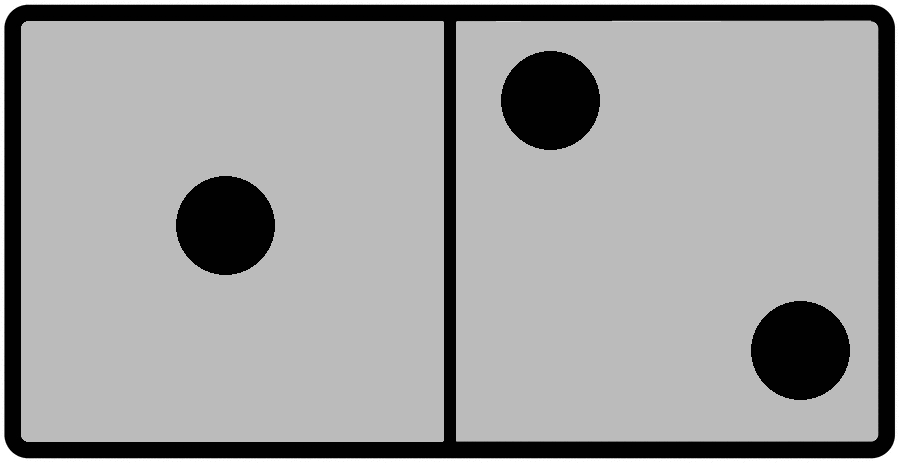
\includegraphics[width=0.2\textwidth]{gray1_2.png}}
\hspace{.1in}
\raisebox{-0.3\height}{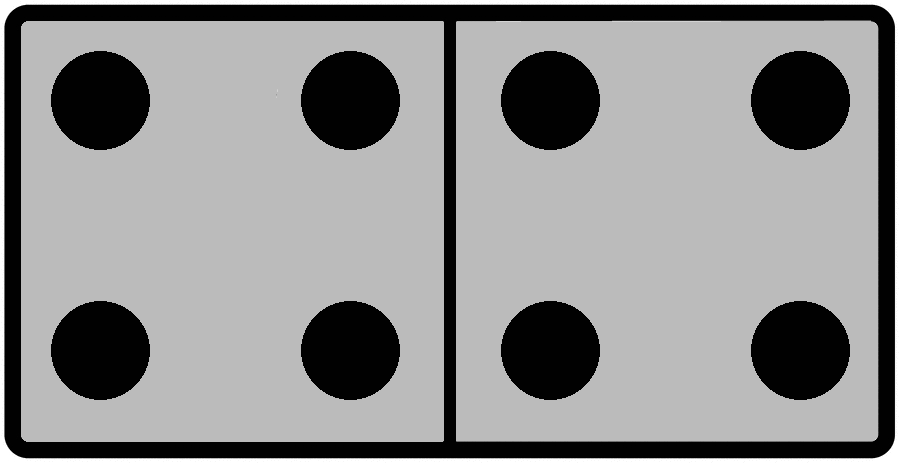
\includegraphics[width=0.2\textwidth]{gray4_4.png}}

Goal domino:
\hspace{1.1in}
\raisebox{-0.3\height}{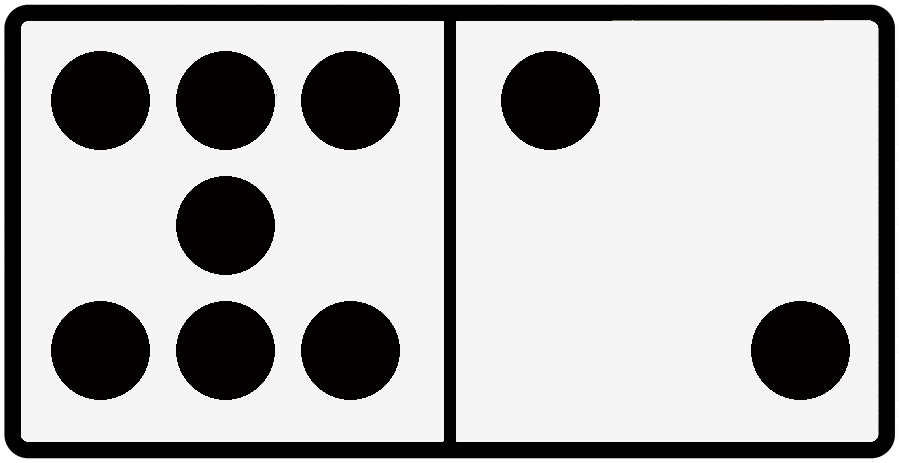
\includegraphics[width=0.2\textwidth]{white7_2.png}}

\footnotesize
(Hint: sometimes you have to go pretty far afield to get a solution, meaning a
large number of one domino and a large \textit{negative} number of the other.)
\normalsize

\item Starter dominoes:
\hspace{.3in}
\raisebox{-0.3\height}{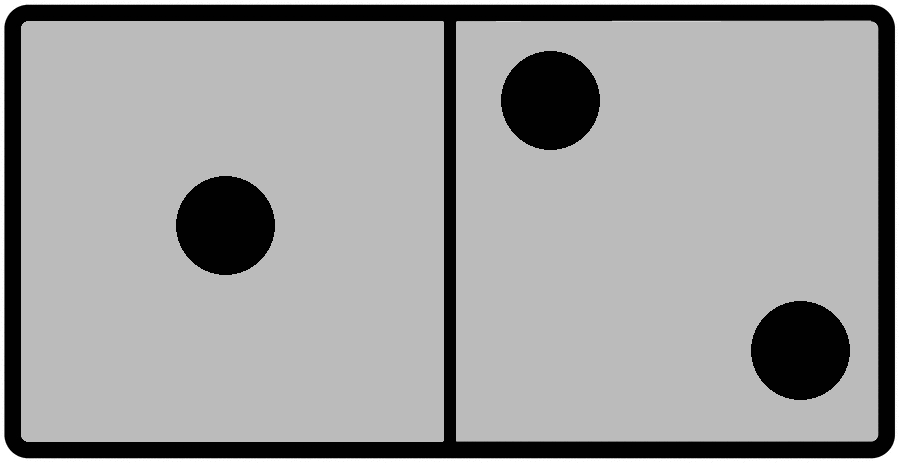
\includegraphics[width=0.2\textwidth]{gray1_2.png}}
\hspace{.1in}
\raisebox{-0.3\height}{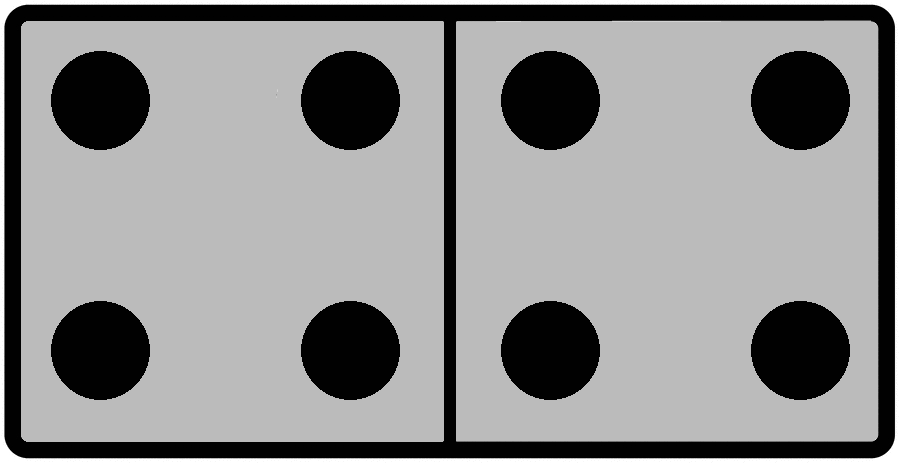
\includegraphics[width=0.2\textwidth]{gray4_4.png}}

Goal domino:
\hspace{1.1in}
\raisebox{-0.3\height}{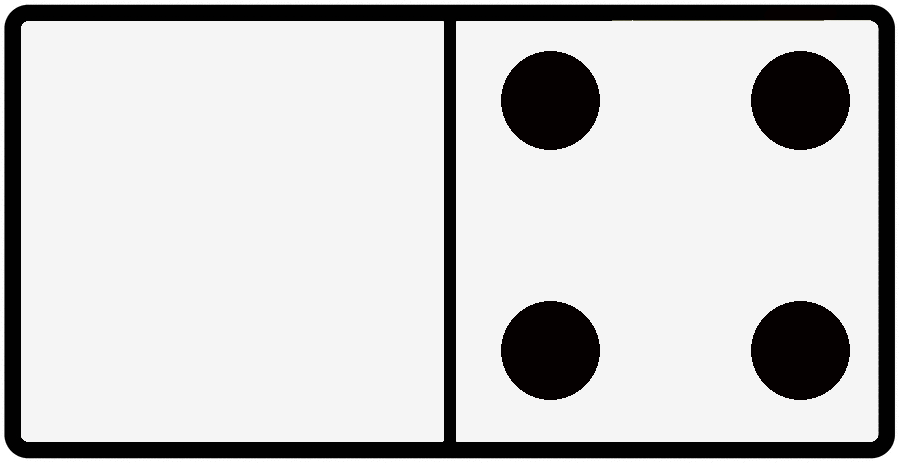
\includegraphics[width=0.2\textwidth]{white0_4.png}}

\footnotesize
(Hint: the goal domino can have a zero on it, just like the starter dominoes
did. But it's really no different; you just have to think creatively about how
to get the numbers to add up to zero on that side.)
\normalsize

\item Starter dominoes:
\hspace{.3in}
\raisebox{-0.3\height}{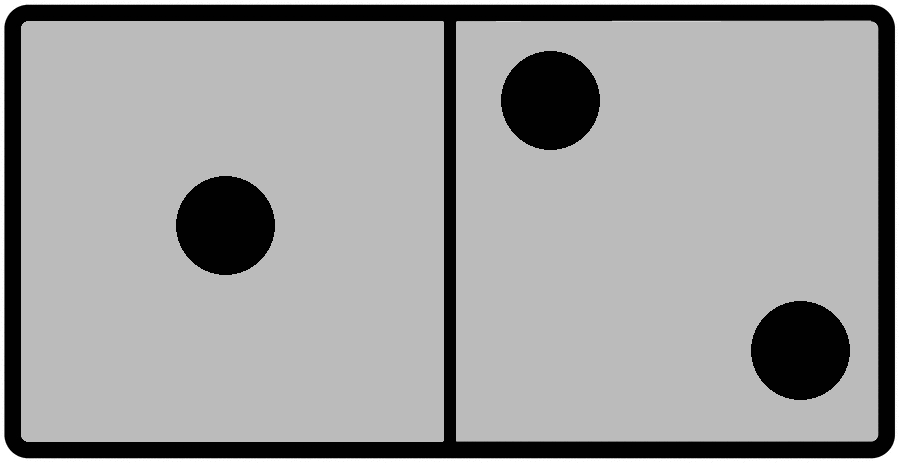
\includegraphics[width=0.2\textwidth]{gray1_2.png}}
\hspace{.1in}
\raisebox{-0.3\height}{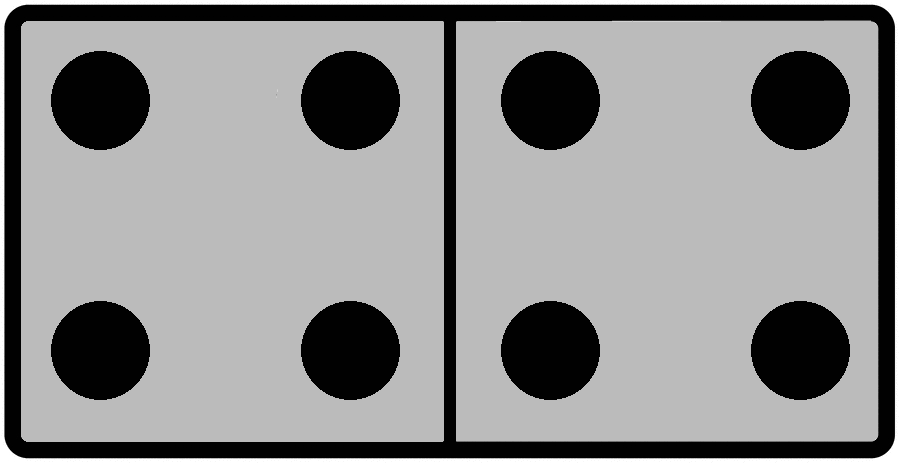
\includegraphics[width=0.2\textwidth]{gray4_4.png}}

Goal domino:
\hspace{1.1in}
\raisebox{-0.3\height}{
\includegraphics[width=0.2\textwidth]{white0_0.png}}

\footnotesize
(Hint: and yeah, the goal domino might even be \textit{completely} zero. That's
really not any different either, and in fact the solution will probably just
jump right off the page at you.)
\normalsize
\label{endDominoPuzzes}
\end{enumerate}

\bigskip
\subsection{Questions for curious minds}

I presume you have tried, and hopefully succeeded at most of these puzzles by
trial and error. Even if you didn't, I hope you've looked at and understood the
solutions I gave at the end of the chapter (p.~\pageref{dominoPuzzleAnswers}).

It's well worth taking a moment after all that fiddling around to consider some
interesting questions:

\begin{enumerate}
\itemsep.1em

\item \label{uniqueSolution} Were your solutions that same as mine in each
case? If so, do you think that was just coincidence? If not, how many different
solutions do you think are possible?

\item \label{alwaysSolveNoMatterGoal} Is it always possible to solve a puzzle
like this, no matter what the \textit{goal} domino is? Or are only a small
number of goal dominoes actually possible to produce?

\item \label{alwaysSolveNoMatterStarters} Is it always possible to solve a
puzzle like this, no matter what the \textit{starter} dominoes are? Or is it
only in a few cleverly crafted scenarios where the numbers happen to work out
just right?

\end{enumerate}

These matters turn out to be at the heart of the subject of linear algebra.
We'll shed light on all of them as we move forward.


\section{The Domino Game, Redux}

I'm now going to give you one more domino puzzle, which is going to seem at
first just like the others. But it turns out that hidden inside is a mystery, a
paradox, a conundrum that will shake our foundations in chapters to come. Here
it is:

\label{blueDominos}
Starter dominoes:
\hspace{.3in}
\raisebox{-0.3\height}{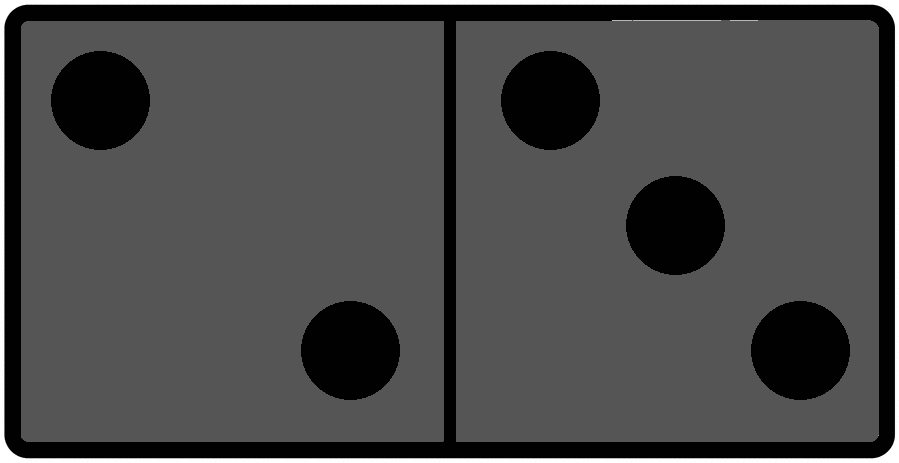
\includegraphics[width=0.3\textwidth]{darkgray2_3.png}}
\hspace{.1in}
\raisebox{-0.3\height}{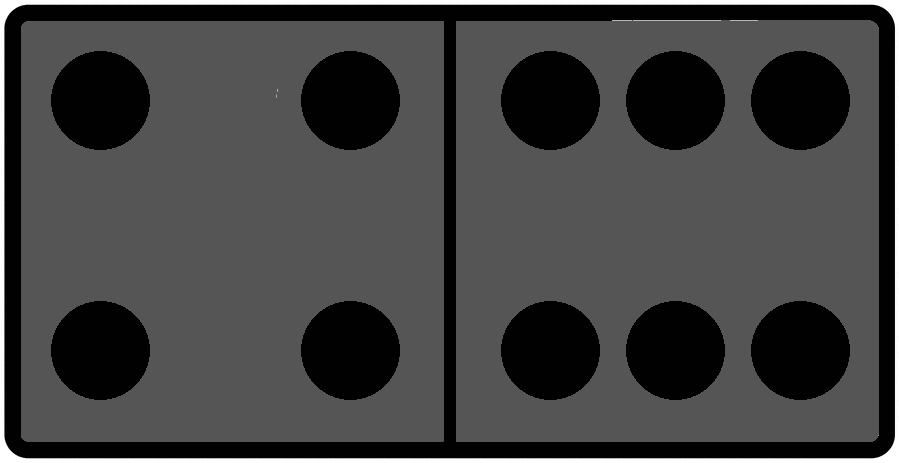
\includegraphics[width=0.3\textwidth]{darkgray4_6.png}}

Goal domino:
\hspace{1.3in}
\raisebox{-0.3\height}{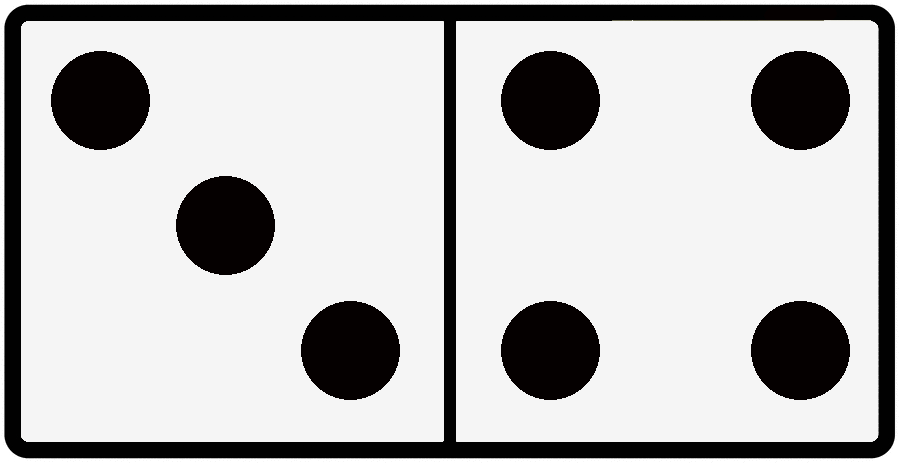
\includegraphics[width=0.3\textwidth]{white3_4.png}}

Our starter dominoes are \textbf{blue}\footnote{Dark gray, actually, since I
made this book black\&white to keep costs down.} instead of yellow this time,
for reasons I'll explain below. Other than that, it's the same kind of problem.
Go ahead -- try it!

I'll mail you \$5 if you can figure it out and send me a solution.

Actually, I'll make it \$5,000.

Don't get too frustrated before you realize the simple truth: it's not
possible.

\subsection{The key point: \underline{\textit{why}} blue dominoes don't work}

You don't have to be too clever to recognize that this whole Domino Game thing
is really math in disguise. And if you haven't seen the connection yet, let me
just point out the following so you can do a face palm:

\begin{compactitem}
\item Dominoes are just two-dimensional vectors.
\item ``Taking some number of the left (or right) domino'' is just
scalar-vector multiplication.
\item Adding together your copies-of-the-left-domino and your
copies-of-the-right-domino is just vector addition.
\end{compactitem}

\index{linear combination}
The central theme of the game is figuring out ``which vectors you can make from
which other vectors.'' The result of ``making'' a new domino is called a linear
combination:

\begin{center}
You get a \textbf{linear combination} of vectors when you multiply each of them
by a scalar and add them up (to yield another vector).
\end{center}

Any vector you can obtain this way is a linear combination of the vectors you
used. The scalars definitely don't have to all be the same. Also, each scalar
can be zero or even negative.

A critical question will turn out to be: what is the complete set of vectors
that are \textit{possible} to get as linear combinations of some ``starter
vectors?'' And to answer that, I'm going to give you a whole new perspective on
dominoes.

\subsection{Dominoes are vectors}

Several of our puzzles involved the yellow starter dominoes 1--2 and 4--4. As I
indicated, dominoes are really vectors in disguise. So I have plotted these two
``dominoes'' in Figure~\ref{fig:yellowVectors}.

\begin{figure}[ht]
\centering
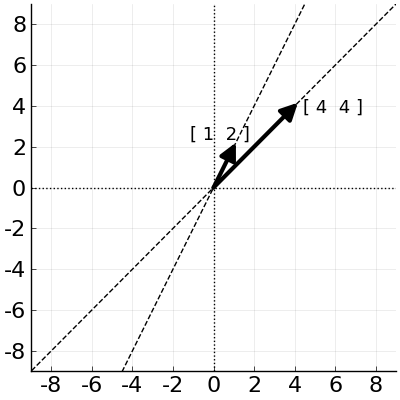
\includegraphics[width=0.8\textwidth]{yellowVectors.png}
\caption{Plotting the dominoes
\protect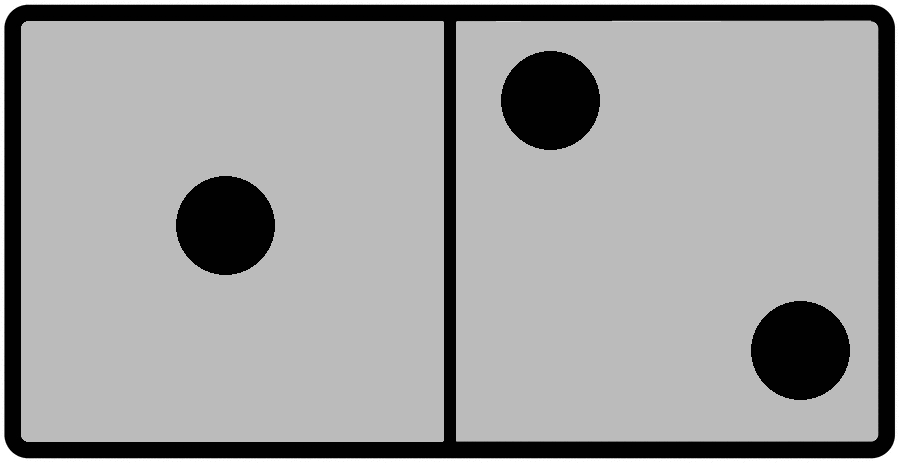
\includegraphics[width=0.07\textwidth]{gray1_2.png} and
\protect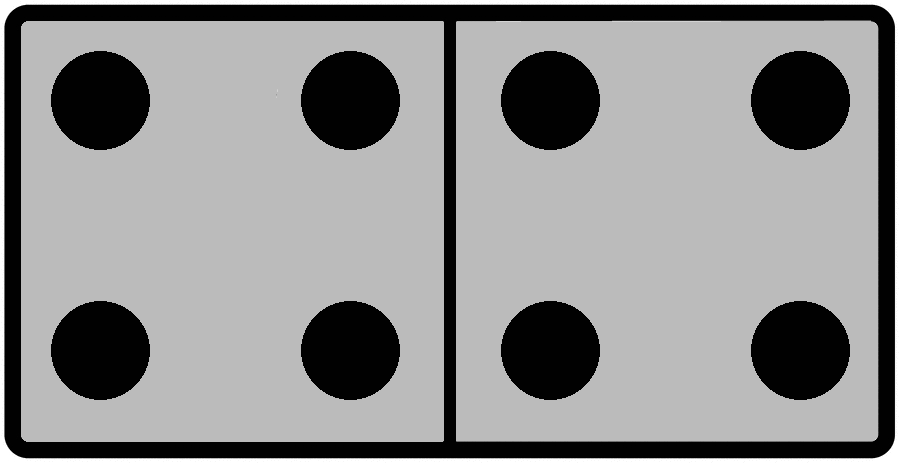
\includegraphics[width=0.07\textwidth]{gray4_4.png} as vectors.}
%\protect{\raisebox{-0.3\height}{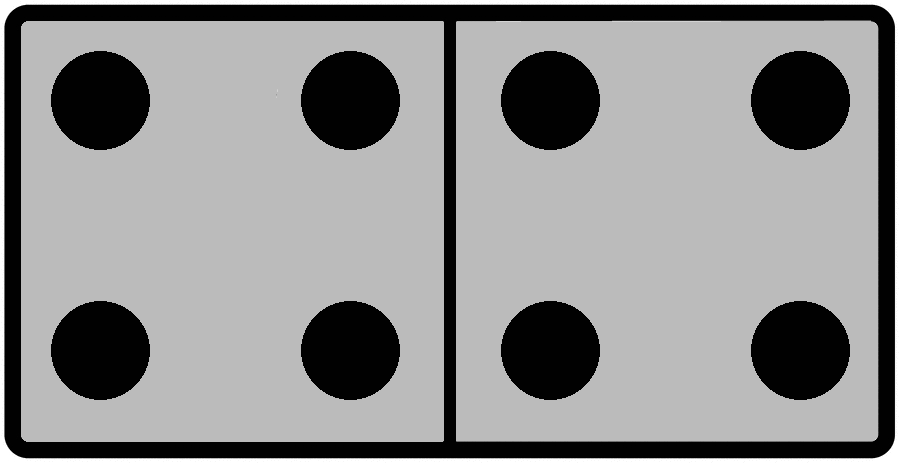
\includegraphics[width=0.05\textwidth]{gray4_4.png}}} as
%vectors.}
\label{fig:yellowVectors}
\end{figure}

Also on the diagram are two dashed lines, each going off to infinity in both
directions. Consider first the steepest of the two lines. It's pointing in
exactly the same direction as the $[\ 1\ \ 2\ ]$ vector. It represents
\textit{all the points you can get to by multiplying that vector by a scalar}.
Take a moment and digest that thought completely. You'll see that some of the
points that dashed line goes through are $(2,4)$, $(4,8)$, $(0,0)$,
$(-\frac{1}{2},-1)$, and $(-4,-8)$. Those points are the tips of the vectors
you would get if you multiplied $[\ 1\ \ 2\ ]$ by 2, 4, 0, $-\frac{1}{2}$, and
$-4$, respectively. Similar comments apply to the dashed line that extends the
$[\ 4\ \ 4\ ]$ vector.

Now consider the process of trying to reach a goal domino like
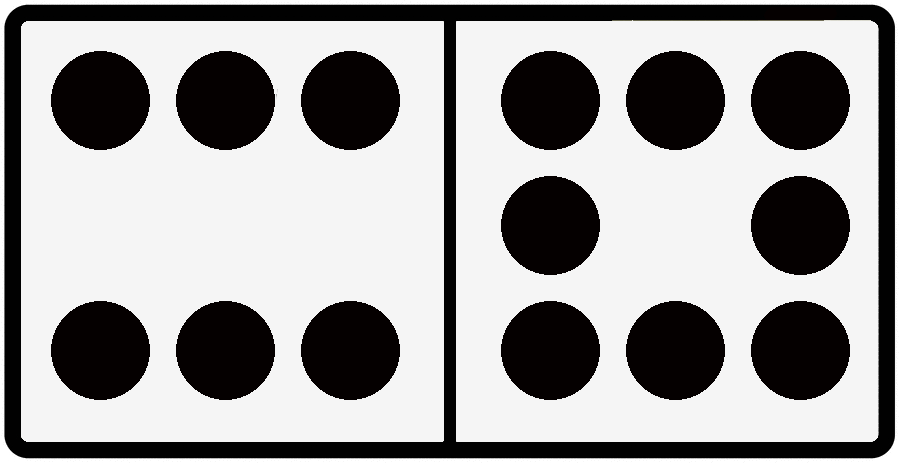
\includegraphics[width=0.06\textwidth]{white6_8.png}, also known as $[\ 6\ \ 8\
]$. What we're effectively asking is: is there any linear combination of $[\ 1\
\ 2\ ]$ and $[\ 4\ \ 4\ ]$ that will reach the point $[\ 6\ \ 8\ ]$? The
setting for this problem is on the left-hand side of 
Figure~\ref{fig:yellowVectors6_8}.

\begin{figure}[ht]
\centering
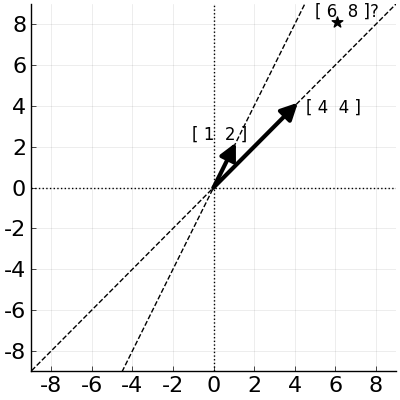
\includegraphics[width=0.44\textwidth]{yellowVectors6_8.png}
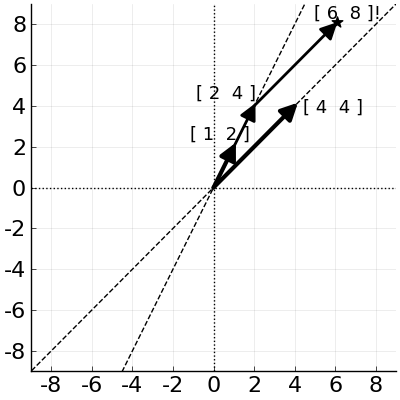
\includegraphics[width=0.44\textwidth]{yellowVectors6_8sol.png}
\caption{Can we reach the point
\protect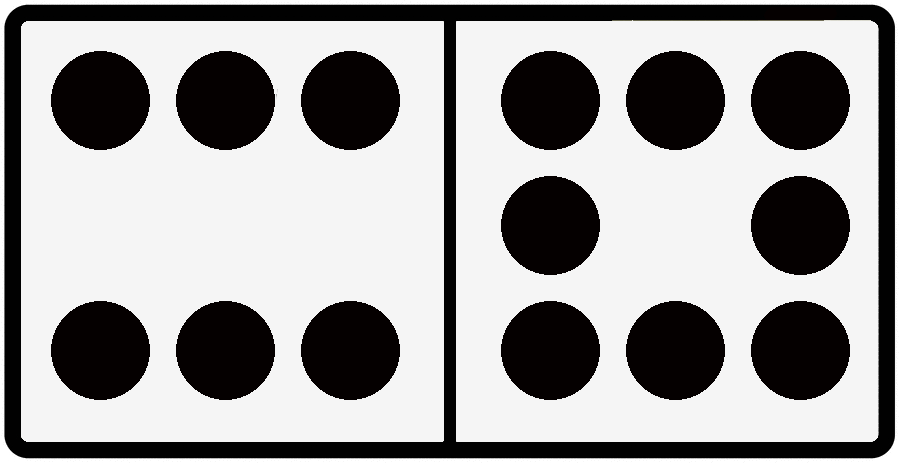
\includegraphics[width=0.06\textwidth]{white6_8.png} (the {\Large
$\star$} at
point $[\ 6\ 8\ ]$) using only multiples of the vectors
\protect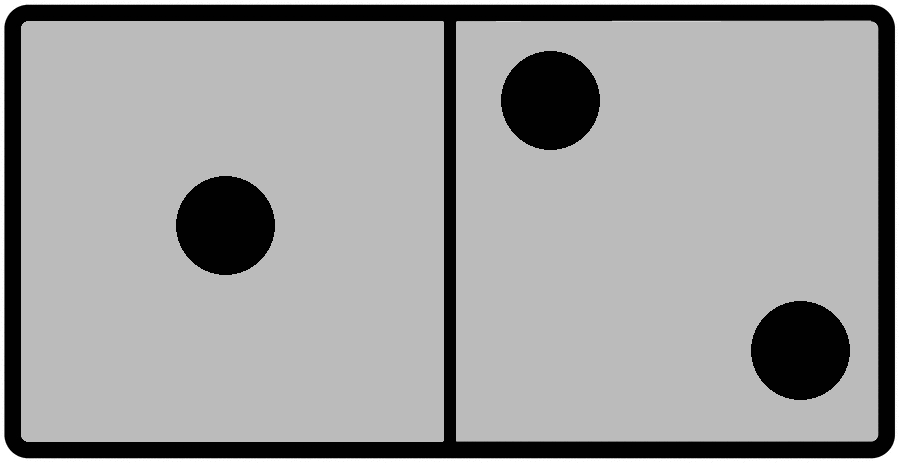
\includegraphics[width=0.06\textwidth]{gray1_2.png} and
\protect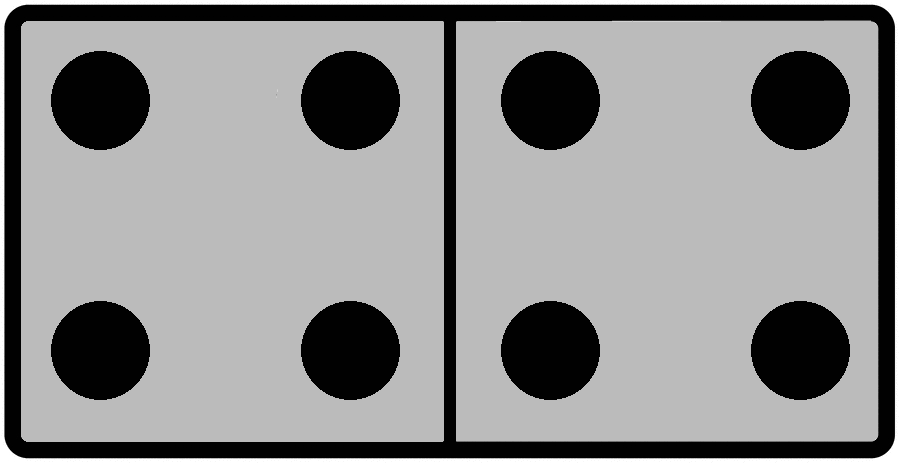
\includegraphics[width=0.06\textwidth]{gray4_4.png}? \textit{Yes!}}
\label{fig:yellowVectors6_8}
\end{figure}

By fiddling around with these numbers Domino-Game-style, you'll hit on the
solution of ``\textbf{two} and \textbf{one}'': two
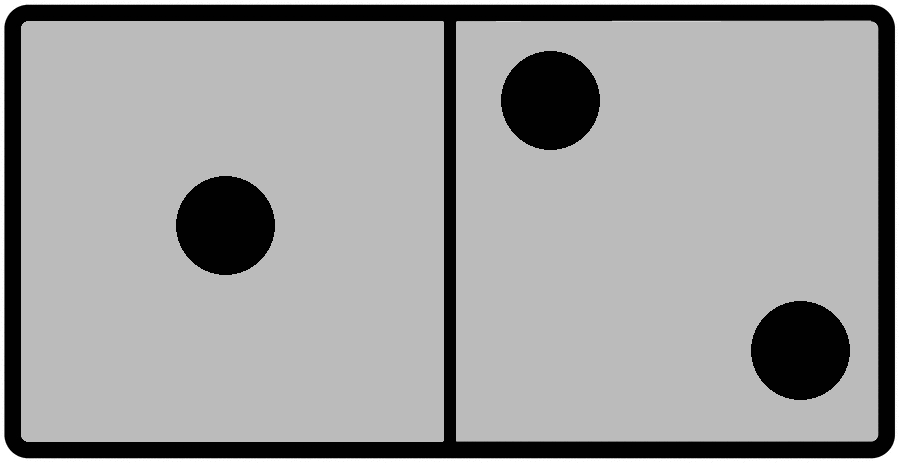
\includegraphics[width=0.06\textwidth]{gray1_2.png} dominoes plus one
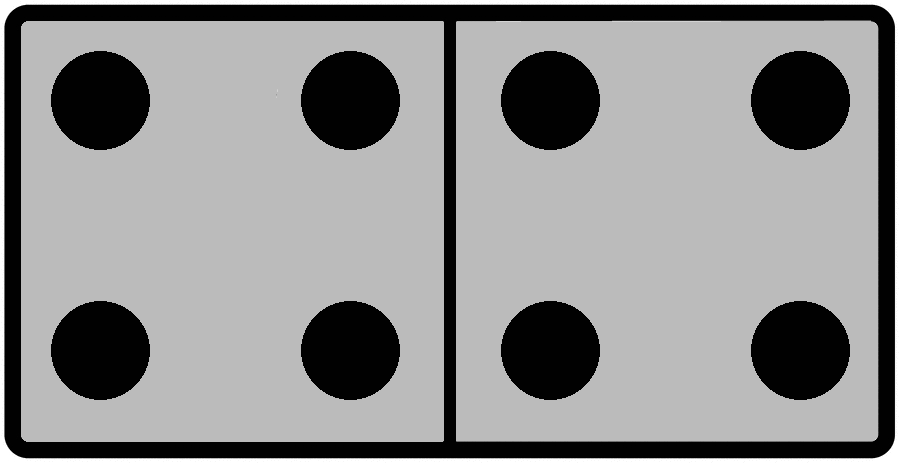
\includegraphics[width=0.06\textwidth]{gray4_4.png} domino gives you a
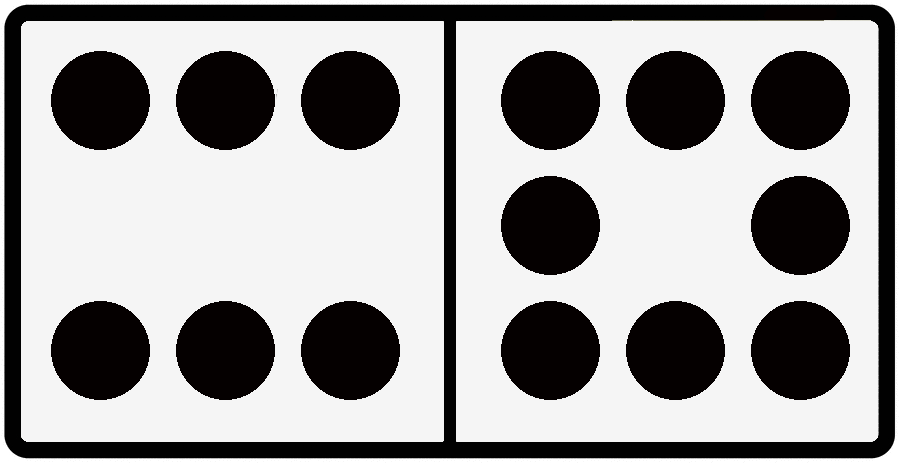
\includegraphics[width=0.06\textwidth]{white6_8.png} domino. That can be
pictured visually on the right-hand side Figure~\ref{fig:yellowVectors6_8}.
Starting at the origin, and moving two times in the direction of the $[\ 1\ \
2\ ]$ vector, we get to the point $[\ 2\ \ 4\ ]$. From there, moving once in
the direction of the $[\ 4\ \ 4\ ]$ vector lands us exactly on the point $[\ 6\
\ 8\ ]$. Voil\`{a}!

\medskip

That was fun -- let's try some more. What about the point $[\ 3\ \ 2\ ]$. Can
we reach \textit{it} by using only multiples of $[\ 1\ \ 2\ ]$ and $[\ 4\ \ 4\
]$?

\index{windshield wiper}
At first glance, it doesn't seem so; after all, the point $(3,2)$ is outside
the ``windshield wiper'' angle between the two dashed lines. But it turns out
we can, if we go against the grain. Moving ``$-1$ times in the $[\ 1\ \ 2\ ]$
direction'' takes us to the point $[\ -1\ \ -2\ ]$. From there, we do
\textit{almost} a complete 180\textdegree. Heading back northeast once in the
$[\ 4\ \ 4\ ]$ direction lands us on $[\ 3\ \ 2\ ]$ as desired. Bingo! (See
Figure~\ref{fig:yellowVectors3_2}.)

\begin{figure}[ht]
\centering
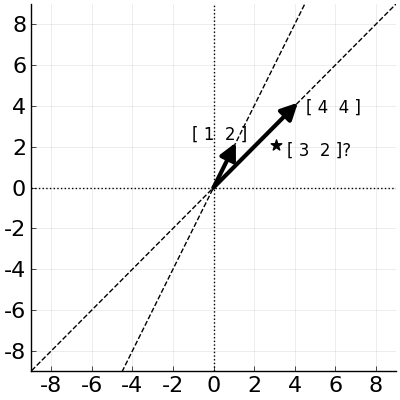
\includegraphics[width=0.44\textwidth]{yellowVectors3_2.png}
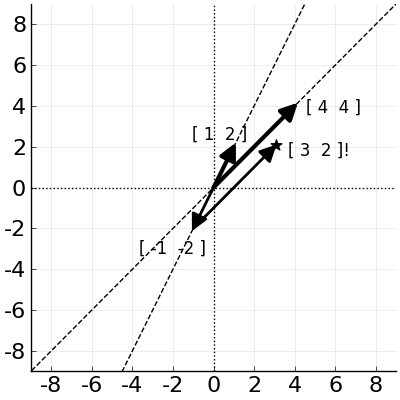
\includegraphics[width=0.44\textwidth]{yellowVectors3_2sol.png}
\caption{Can we reach the point $[\ 3\ \ 2\ ]$ using only $[\ 1\ \ 2\ ]$ and
$[\ 4\ \ 4\ ]$? \textit{Yes!}}
\label{fig:yellowVectors3_2}
\end{figure}

\index{backwards}
And how about $[\ 0\ \ 4\ ]$? This time it's the 
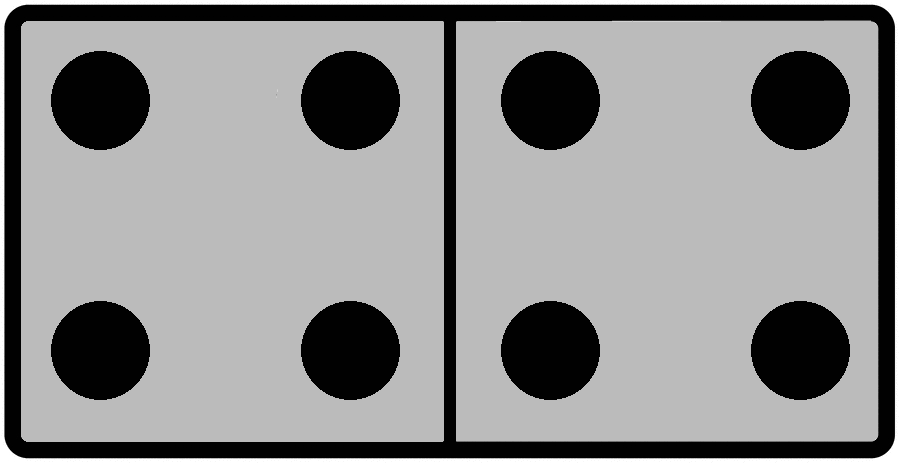
\includegraphics[width=0.06\textwidth]{gray4_4.png} domino that we use
``backwards.'' Going four times in the $[\ 1\ \ 2\ ]$ direction followed by
$-1$ in the $[\ 4\ \ 4\ ]$ direction gives us the solution ``4 \& $-1$,'' as
depicted in Figure~\ref{fig:yellowVectors0_4}.

\begin{figure}[hb]
\centering
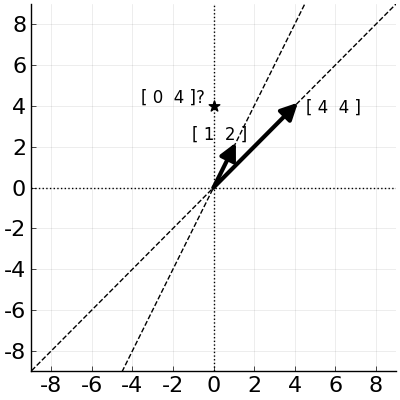
\includegraphics[width=0.44\textwidth]{yellowVectors0_4.png}
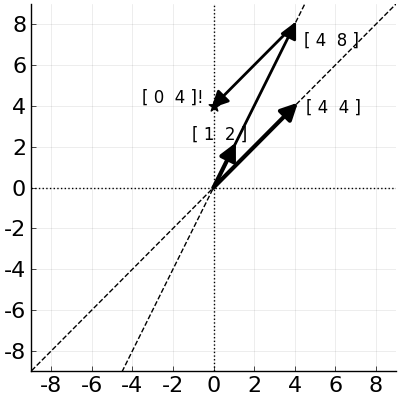
\includegraphics[width=0.44\textwidth]{yellowVectors0_4sol.png}
\caption{Can we reach the point $[\ 0\ \ 4\ ]$ using only $[\ 1\ \ 2\ ]$ and
$[\ 4\ \ 4\ ]$? \textit{Yes!}}
\label{fig:yellowVectors0_4}
\end{figure}

At this point, you'll probably guess what I'm going to say next. Yes indeed,
\textit{any} point in the entire $x,y$ plane can be reached through some
combination of the $[\ 1\ \ 2\ ]$ and $[\ 4\ \ 4\ ]$ vectors. And that gives us
the answer to one of our questions from p.~\pageref{alwaysSolveNoMatterGoal}
(question \#\ref{alwaysSolveNoMatterGoal}): surprisingly, \textit{yes} we can
always find a solution to the Domino Game puzzle, no matter what the goal
domino is. Amazing!

Most of my students are as surprised by that result as I was back in the day.
When I first give them Domino puzzles, they figure, ``okay, Stephen has
specially concocted a case where it just happens to work out that I can combine
the two yellow dominoes into a white one somehow. I'll work his special puzzle
and come up with the slick answer.'' Little do they realize that \textit{any}
white domino whatsoever is solvable; I didn't have to come up with anything
special at all.

\smallskip

Now the second lesson of these vector pictures may be harder to see. It's the
answer to question \#\ref{uniqueSolution} from p.~\pageref{uniqueSolution}. Not
only can every Domino problem be solved, but \textit{it can be solved in only
one way.}

If you did it right, your answers to the six puzzles on
pp.~\pageref{startDominoPuzzles}-\pageref{endDominoPuzzes} were exactly the
same as mine on p.~\pageref{dominoPuzzleAnswers}. Perhaps that struck you as a
coincidence at first: ``gee, it's sure funny that I always keep hitting on the
exact same solution that Stephen did!'' But if you stare at
Figure~\ref{fig:yellowVectors6_8} and friends, you might see the reason.
Starting from the origin, and striking out in the first vector's direction, you
only have one choice if you want to get to the right place. In
Figure~\ref{fig:yellowVectors6_8}'s case, you \textit{must} stop at $[\ 2\ \ 4\
]$. If you stop earlier, or later, then you're destined to miss the mark: going
in the $[\ 4\ \ 4\ ]$ direction from anywhere else you might stop won't land
you at exactly $[\ 6\ \ 8\ ]$.

\subsection{But...}

So every point is reachable, and is reachable in only one way. But that's only
\textit{\underline{if}} you have yellow starter dominoes. If you've got blue
ones, it's a totally different story.

\begin{figure}[ht]
\centering
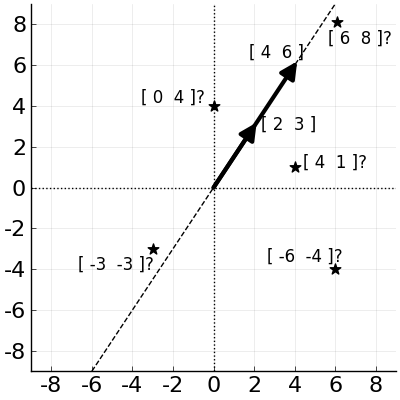
\includegraphics[width=0.7\textwidth]{blueVectors.png}
\caption{Can we reach the points
$[\ 6\ \ 8\ ]$,
$[\ 0\ \ 4\ ]$,
$[\ 4\ \ 1\ ]$,
$[\ -6\ \ -4\ ]$,
$[\ -3\ \ -3\ ]$...or virtually anything else
using only $[\ 2\ \ 3\ ]$ and $[\ 4\ \ 6\ ]$? \textbf{No.}}
\bigskip
\label{fig:blueVectors}
\end{figure}

Figure~\ref{fig:blueVectors} shows the hopeless situation. The telltale sign of
misery is that \textit{there's only one dashed line.} The 
{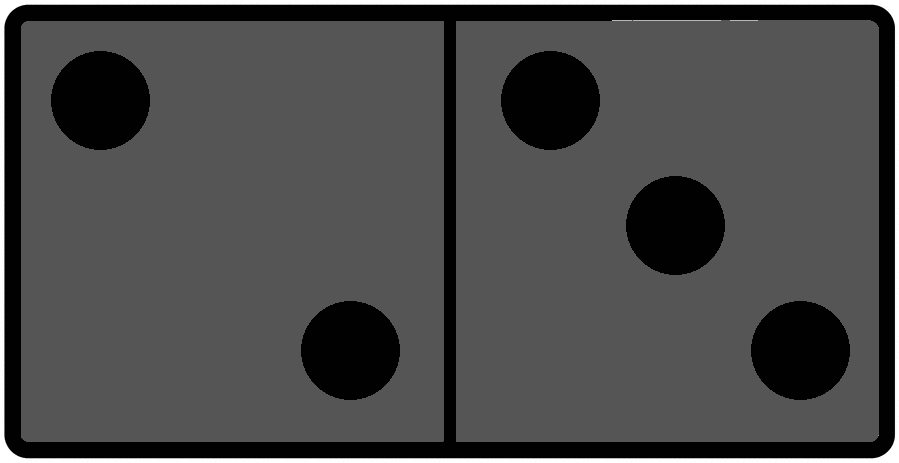
\includegraphics[width=0.06\textwidth]{darkgray2_3.png}} and
{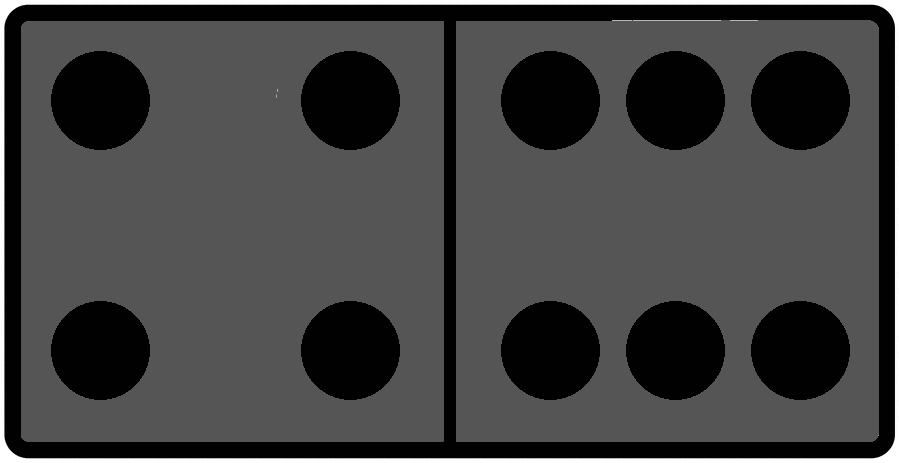
\includegraphics[width=0.06\textwidth]{darkgray4_6.png}} vectors point in
\textit{exactly} the same direction, so no matter how hard we try, there's no
getting off that one line. In the middle of a promising two-dimensional
landscape, we're stuck in a one-dimensional sub-world.


\section{Linear independence in two dimensions}

\index{linear independence}

The yellow {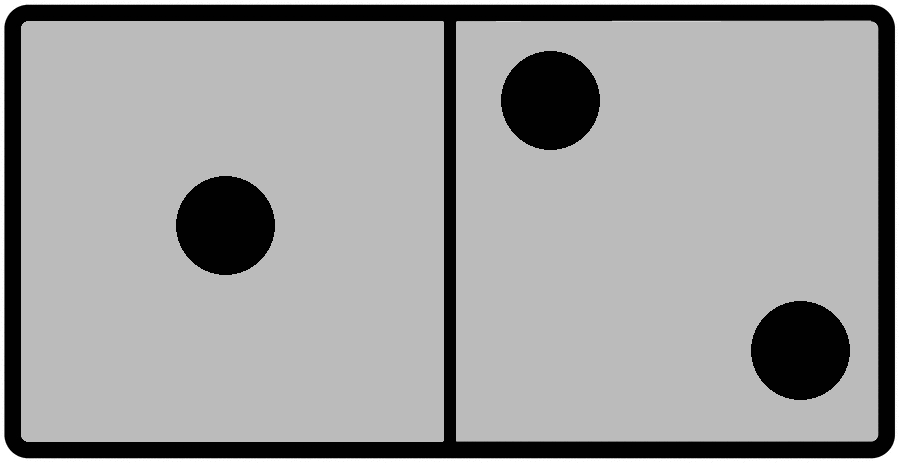
\includegraphics[width=0.06\textwidth]{gray1_2.png}} and
{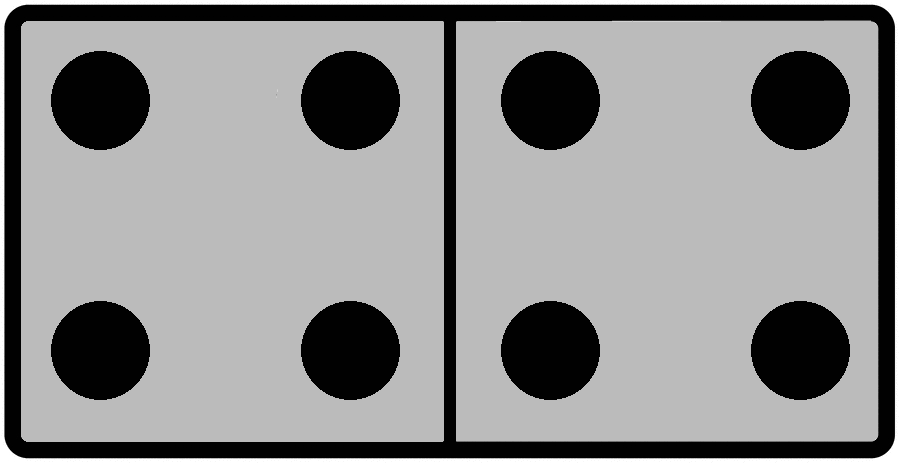
\includegraphics[width=0.06\textwidth]{gray4_4.png}} vectors are called
\textbf{linearly independent}. By contrast, the blue
{\includegraphics[width=0.06\textwidth]{darkgray2_3.png}} and
{\includegraphics[width=0.06\textwidth]{darkgray4_6.png}} vectors are
\textbf{linearly dependent}. Figure~\ref{fig:dominoFacts}
(p.~\pageref{fig:dominoFacts}) sums up some
extremely important facts about these two cases in one handy table. Let me
explain each item in turn.

\vspace{-.2in}

\begin{itemize}
\itemsep.1em

\item \textbf{Yellow dominoes are linearly independent.} This means they point
in different directions, so that each one gives you a ``fresh'' degree of
freedom to travel in.

% DANGER: "up" to refer to figure

\item \textbf{You can't get one yellow domino from the other.} A corollary of
the ``different directions'' thing is that if you tried to get to the tip of
the first yellow domino using only the second, you couldn't do it. Look back at
Figure~\ref{fig:yellowVectors} (p.~\pageref{fig:yellowVectors}) if you don't
believe me. From the origin, can you get to the point $[\ 1\ \ 2\ ]$ going only
in the $[\ 4\ \ 4\ ]$ direction? No. But if you look up at
Figure~\ref{fig:blueVectors} you'll see that you \textit{can} do it with our
blue dominoes. Can you get to $[\ 2\ \ 3\ ]$ using only the $[\ 4\ \ 6\ ]$
vector? Sure, just take half of it.

Another way to think of it is that if you have blue dominoes, one of them is
superfluous. Say you have $[\ 2\ \ 3\ ]$, and I come along trying to sell you
$[\ 4\ \ 6\ ]$ as well. Why bother? You can already go in that direction! Heck,
you can produce $[\ 4\ \ 6\ ]$ yourself just by doubling the domino you already
have.


\item \textbf{Yellow dominoes are the common case.} Suppose I picked two
dominoes out of a bag and put them in front of you. Are they more likely to be
yellow, or blue? A moment's consideration will tell you the answer is yellow.
The only way the dominoes can be blue is if they point in
\underline{\textit{exactly}} the same direction. The odds of that are
fantastically small.

Think of it this way. Let's say the first domino out of the bag is $[\ 1\ \ 3\
]$. And let's say the left half of the second domino is 4, so that the second
domino is $[\ 4\ \ ?\ ]$. Think about what would have to happen for the pair of
dominoes to be blue. That question mark would have to be exactly 12.
\textit{Only} 12. Absolutely any other number for the question mark would give
you yellow dominoes.

\item \textbf{With yellow dominoes, you can get \textit{any} white domino.}
This is perhaps the most important point. The yellow dominoes have enough
coverage that any point in the entire plane is reachable using them. The sorry
blue dominoes, on the other hand, are inbred; you can't get anywhere on the
plane except the points along their shared, lonely line.

\item \textbf{With yellow dominoes, each solution is unique.} This may or may
not have been obvious to you from the diagrams, but I promise it's so. You can
reach each point in only one way. By contrast, everything the blue dominoes can
reach -- which admittedly, ain't much -- can be reached in multiple ways
(including the origin; see the next point).

\index{trivial@``trivial'' solution}
\label{trivialSolution}

\item \textbf{Yellow dominoes can't get to the origin, except ``trivially.''}
One last point is that with yellow dominoes, the only way to get to the origin
is to take zero of the first domino and zero of the second. (This is called a
\textbf{trivial solution}.) That's because once you set out in the first
domino's direction, using the second one has to take you in a
\textit{different} direction, and hence not back to where you came. With blue
dominoes, you can do this in many different ways: take six $[\ 2\ \ 3\ ]$'s
minus three $[\ 4\ \ 6\ ]$'s, or $-1$ $[\ 2\ \ 3\ ]$'s and half a $[\ 4\ \ 6\
]$, \textit{etc.} I guess that's some small recompense for having to stay on
that one line: blue dominoes truly \textit{own} that line and can tread it to
their heart's content. This seemingly obscure fact will actually play a
surprising role later on.

\end{itemize}

By the way, a student once asked me, ``what if you get one yellow domino and
one blue? What happens then?'' Perhaps you'll see the answer immediately as one
of my other students did. The answer is \textit{that can't happen.} No domino
is, by itself, intrinsically yellow or blue: it's only yellow or blue
\textit{with respect to another one.} It's the \textit{pair} of dominoes that
are yellow if they point in different directions, or blue if they point in the
same direction.


\begin{figure}[ht]
\begin{framed}
\begin{center}
\small
\hspace{-.2in}
\begin{tabular}{l|r}
Yellow dominoes \ 
\raisebox{-0.25\height}{\includegraphics[width=0.07\textwidth]{gray1_2.png}} 
\raisebox{-0.25\height}{\includegraphics[width=0.07\textwidth]{gray4_4.png}} &
\raisebox{-0.25\height}{\includegraphics[width=0.07\textwidth]{darkgray2_3.png}} 
\raisebox{-0.25\height}{\includegraphics[width=0.07\textwidth]{darkgray4_6.png}} 
\ Blue dominos \smallskip \\
\hline \\ 
linearly \textbf{independent} & linearly \textbf{dependent} \\
can't get any yellow from others & 
can get each blue from others \\
``common'' & ``rare'' \\
can make \textit{any} white domino & can make only a few \\
each goal reachable in one way & each goal reachable \textit{many} ways \\
can only get
\raisebox{-0.3\height}{\includegraphics[width=0.07\textwidth]{white0_0.png}} 
``trivially" &
can get 
\raisebox{-0.3\height}{\includegraphics[width=0.07\textwidth]{white0_0.png}}
in many ways \\
\end{tabular}
\end{center}
\end{framed}
\vspace{-.2in}
\caption{Important domino facts.}
\label{fig:dominoFacts}
\end{figure}

\section[Linear independence in more dimensions]{\large Linear independence in more dimensions}

Now I wish things could stay that easy but they just can't. When we move to
three dimensions (and beyond) things become more subtle, even besides being
harder to visualize.

First let's look at an easy case. Suppose you have the three ``triominoes'' $[\
1\ 2\ 3\ ]$, $[\ -4\ 0\ 1\ ]$, and $[\ 2\ 4\ 6\ ]$. You can probably eyeball
those and see that they are \textit{not} linearly independent, because the
first and third dominoes are multiples of each other. (Multiply $[\ 1\ 2\ 3\ ]$
by 2 and you get $[\ 2\ 4\ 6\ ]$.) And if you can get one vector from one of
the others, that's the death knell for our yellow hopes and dreams: These
vectors are unavoidably blue.

In three dimensions, blue triominoes mean that we can't get to every point in
three-dimensional \textbf{space} just by using those vectors. That's hard to
visualize, but if you can picture the following, you'll get the idea. Recall
that in 2-d, blue vectors sat on the same dashed line. You couldn't get to the
rest of the plane. In 3-d, blue vectors all sit on the same \textit{plane}. You
can get anywhere on that two-dimensional surface, but not anywhere else in the
vastness of three-dimensional space.

Perhaps this is easier to see if I change the example. Suppose my three
triominoes are $[\ 4\ 2\ 0\ ]$, $[\ 2\ 3\ 0\ ]$, and $[\ 6\ 5\ 0\ ]$. Now you
can add multiples of these three vectors together all day, but you'll never get
a third entry other than zero. I can't get to a point like $[\ 4\ 3\ 7\ ]$,
because how would I ever get a 7 in the third slot? All the vectors I have to
work with have a zero there!

In picture terms, if we consider the coordinates to be $x$, $y$, and $z$, where
the $z$ axis goes ``in'' and ``out'' of the page, those three vectors let us
reach only the points \textit{on} the flat page. All the points in space that
are in front of the page, or behind the page, are out of reach.

\smallskip

I promise you the same basic thing is true for $[\ 1\ 2\ 3\ ]$, $[\ -4\ 0\ 1\
]$, $[\ 2\ 4\ 6\ ]$ example. It's only harder to see in your mind's eye because
in this case, the plane we're trapped on isn't flat. It's angled through space,
slicing slant-wise through the origin. But it's still true that the vast
majority of 3-d points can't be reached. The problem here, just like with blue
dominoes, is that one of the vectors in the list (the third one) doesn't give
us any power we didn't already have with one of the others (the first one).

\medskip

Now so far, this seems just the same as the two-dimensional case, except that
we have three entries per vector to work with. But unfortunately, even if none
of the three vectors is a multiple of any of the other, that's \textit{not}
enough to guarantee linear independence. Three vectors which are ``pairwise
independent'' from each other -- meaning $\overrightarrow{v_1}$ is not a
multiple of $\overrightarrow{v_2}$, nor $\overrightarrow{v_2}$ of
$\overrightarrow{v_3}$, nor $\overrightarrow{v_3}$ of $\overrightarrow{v_1}$ --
can still be a linearly dependent set.

\index{linear combination}

How? \textit{If one is a linear combination of the other two.} Consider these
three vectors:

\begin{center}
\begin{tabular}{rlrrrl}
$\overrightarrow{v_1}$ &= [\ & 2\ & 0\ & $-3$\ & ] \\
$\overrightarrow{v_2}$ &= [\ & $-1$\ & 4\ & 4\ & ] \\
$\overrightarrow{v_3}$ &= [\ & 3\ & 4\ & $-2$\ & ] \\
\end{tabular}
\end{center}

Those look pretty linearly independent to me. But they're not. If you take
twice the first vector plus the second vector, you get the third vector:

\begin{align*}
2 \overrightarrow{v_1} + 1 \overrightarrow{v_2} &=
[\ 4\ \ 0\ \ -6\ ] + [\ -1\ \ 4\ \ 4\ ] = [\ 3\ \ 4\ \ -2\ ] = \overrightarrow{v_3} \\
\end{align*}

As before, then, the third vector \textit{didn't give us any additional power.}
If we wanted to move in the $[\ 3\ 4\ -2\ ]$ direction, we could do so using
only vectors $\overrightarrow{v_1}$ and $\overrightarrow{v_2}$ in the right
quantities. The offer of that $\overrightarrow{v_3}$ vector leaves us with an
awkward pause and saying as politely as possible ``no, thanks.''

Now finally, we're ready for our supreme definition of linear independence, no
matter how many dimensions. Here goes:

\begin{framed}
A set of vectors is \textbf{linearly independent} only if none of them can be
made from a linear combination of the others.
\end{framed}

If you're given a set of vectors, and you can find a superfluous one in the
bunch, remove it so you whittle the set down to size. When you get to the point
where none of the remaining vectors can be deleted without losing the ability
to reach some points, then you know you have a linearly independent set.

\section{Foundational definitions}

We close this heady chapter by defining a few more crucial terms that we'll
make use of again and again.

\index{vector space}

\begin{framed}
A ``\textbf{vector space}'' is a world of $n$ dimensions in which
$n$-dimensional vectors live. (like the $x$-$y$ plane, or the 3-d space.)
\end{framed}

I hinted at this term back on p.~\pageref{vectorSpace}, and mentioned that it's
sometimes used in a very abstract way. The above definition, believe it or not,
is a pretty brass-tacks definition, since we're defining it in terms of
dimensions and coordinates. Just think of a ``vector space'' as ``the place
where vectors (of a particular length) live'' and you won't be too far off.

\index{span}
\begin{framed}
The set of \textit{all} linear combinations of a set of vectors is called the
\textbf{span} of that set.
\end{framed}

This is precisely the question of ``where can I \textit{get} using these
starter dominoes?'' that we asked in the Domino Game. I can combine starter
vectors with each other in numerous ways to get other vectors. If I kept doing
that and doing that infinitely, what is my \textit{entire} set of possible
vacation spots? Answer: the \textbf{span}.

To be concrete:

\vspace{-.15in}
\begin{itemize}

\item The span of \{ 
\raisebox{-0.25\height}{\includegraphics[width=0.07\textwidth]{gray1_2.png}},
\raisebox{-0.25\height}{\includegraphics[width=0.07\textwidth]{gray4_4.png}}
\} is \textbf{the whole $x$-$y$ plane}.

\item The span of \{
\raisebox{-0.25\height}{\includegraphics[width=0.07\textwidth]{darkgray2_3.png}},
\raisebox{-0.25\height}{\includegraphics[width=0.07\textwidth]{darkgray4_6.png}}
\}, on the other hand, is merely \textbf{the line through the origin with slope
$\frac{3}{2}$} (``rise over run'').


% TODO: *Do* we actually show how to verify a set of vectors is linearly indep?

\item The span of \{ $[2 \ 3 \ 1],\  [0 \ -9 \ 0], \ [0 \ 1 \ 1]$ \} is
\textbf{the whole three-dimensional $x$-$y$-$z$ space}, since that set is
linearly independent. (You can believe me or not, but it is. We'll figure out
how to verify that later on.)

\item The span of \{ $[2 \ 0 \ -3],\  [-1 \ 4 \ 4],\  [3 \ 4 \ -2]$ \} is
\textit{not} the whole $x$-$y$-$z$ space, since as we learned above, that set
is not linearly independent. Its span is merely \textbf{a 2-d plane slicing
through the origin} of three-dimensional space.

\end{itemize}


\index{basis}
\label{basis}

\begin{framed}
A \textbf{basis} for a vector space is a \textit{linearly independent} set of
vectors that \textit{spans} the space.
\end{framed}

Note that two-part definition. Your vectors have to (1) be independent of one
another, and (2) span the entire space. Only then do they constitute a basis.

Important fact: if you have a basis, then every vector in the entire vector
space can be expressed as a linear combination of the basis vectors in exactly
one way.

For example, we saw that \{ $[\ 1\ \ 2\ ]$, $[\ 4 \ \ 4\ ]$ \} was a basis for
the $x$-$y$ plane. Therefore, every point on the $x$-$y$ plane can be formed by
a unique linear combination of those vectors:

\begin{align*}
[\ 6 \ \ 8\ ]\ &=\ 2\ [\ 1 \ \ 2\ ] \ + \ 1\ [\ 4 \ \ 4\ ] \\
[\ 0 \ \ 4\ ]\ &=\ 4\ [\ 1 \ \ 2\ ] \ - \ 1\ [\ 4 \ \ 4\ ] \\
[\ 4 \ \ -4\ ]\ &=\ -8\ [\ 1 \ \ 2\ ] \ + \ 3\ [\ 4 \ \ 4\ ] \\
\end{align*}
\vspace{-.7in}
\begin{center}
\textit{etc.}
\end{center}

We'll look at this in a new and deep way later on, but you can begin to grasp
it now: using a basis kind of gives us \textit{a new coordinate system} in
which to express a vector. For example, as shown above, the vector $[\ 4\ \ -4\
]$ can be expressed as \textbf{--8} of the $[\ 1\ \ 2\ ]$ vector plus
\textbf{3} of the $[\ 4\ \ 4\ ]$ vector. That means that its coordinates are
kinda sorta ``$(-8,3)$'' in this basis rather than ``$(4,-4)$'' in the original
basis. Dude, that's mind-blowing.

\index{basis}
\index{standard basis}
\begin{framed}
The ``\textbf{standard basis}'' is a basis whose vectors have norm 1 and which
point in each axis direction.
\end{framed}

In other words:

\begin{compactitem}

\item In two dimensions, the standard basis is the vectors $[\ 1\ \ 0\ ]$ and
$[\ 0\ \ 1\ ]$.

\item In three dimensions, it's the vectors $[\ 1\ \ 0\ \ 0\ ]$, $[\ 0\ \ 1\ \
0\ ]$, and $[\ 0\ \ 0\ \ 1\ ]$.

\item In four dimensions, it's the vectors $[\ 1\ \ 0\ \ 0\ \ 0\ ]$, $[\ 0\ \ 1\ \
0\ \ 0\ ]$, $[\ 0\ \ 0\ \ 1\ \ 0\ ]$, and $[\ 0\ \ 0\ \ 0\ \ 1\ ]$.

\item \textit{Etc.}
\end{compactitem}


\smallskip
Note that in the standard basis, we have:

\vspace{-.3in}
\begin{align*}
[\ 6 \ \ 8\ ]\ &=\ 6\ [\ 1 \ \ 0\ ] \ + \ 8\ [\ 0 \ \ 1\ ] \\
[\ 0 \ \ 4\ ]\ &=\ 0\ [\ 1 \ \ 0\ ] \ + \ 4\ [\ 0 \ \ 1\ ] \\
[\ 4 \ \ -4\ ]\ &=\ 4\ [\ 1 \ \ 0\ ] \ - \ 4\ [\ 0 \ \ 1\ ] \\
\end{align*}
\vspace{-.7in}
\begin{center}
\textit{etc.}
\end{center}

Thus in some ways, the standard basis is sort of the ``natural'' coordinate
system. (Hang on to your hats in Chapter~\ref{ch:eigen}, though, when we
consider a different ``natural'' one.)

Fact: all possible bases for a vector space have the \textit{same} number of
vectors in them. Why? Well, you can't span the space with any fewer. And you
can't be linearly independent if you have any more. So no matter what basis you
tell me you have for the $x$-$y$ plane, I know it'd better have exactly two
vectors in it or you're a liar. If you tell me you have a basis for 
$x$-$y$-$z$ space, it'd better have three vectors in it: no more, and no fewer.

\medskip

Last one, which you might already be able to guess:

\index{dimension}
\begin{framed}
The \textbf{dimension} of a vector space is the number of elements in a basis
for it.
\end{framed}

We've talked about the dimension of a \textit{vector} before, but not of a
vector space. The dimension of a vector space is how many vectors are required
to get everywhere in it. And that in turn is simply the dimension of the
vectors that live in it. It's no accident that for \textit{three}-dimensional
space, a basis has \textit{three} vectors with \textit{three} elements each.


\section{Changing bases}

If each basis is merely a new coordinate system in which to express vectors, we
ought to be able to change between bases at will. And in fact we can. Let's see
how.

\subsection{Changing \textit{to} the standard basis}

\label{changeOfBasis}
\index{Ron}
\index{domino basis}

Ron has a two-dimensional vector called $\overrightarrow{\textbf{r}}$. I'll
tell you that its coordinates are $3$ and $-1$, BUT before you try to visualize
it, there's a catch: these coordinates are \textit{not} expressed in the
standard basis, but in the ``\textit{domino basis}'' we've used several times
in this chapter:
\raisebox{-0.25\height}{\includegraphics[width=0.07\textwidth]{gray1_2.png}}
{\Large /}
\raisebox{-0.25\height}{\includegraphics[width=0.07\textwidth]{gray4_4.png}}.

This is the first time I've used the phrase ``expressed as coordinates in a
certain basis,'' because up until now, we've always been implicitly assuming
the standard basis. If I said a vector had components ``7'' and ``4,'' it has
gone without saying that I meant ``7 units in the $[\ 1\ \ 0\ ]$ direction, and
4 units in the $[\ 0\ \ 1\ ]$ direction.'' Viewed in this way, a vector with
coordinates 7 and 4 is really a linear combination of the two (standard) basis
vectors:

\vspace{-.15in}
\begin{align*}
7 \cdot \begin{bmatrix} 1 \\ 0 \\ \end{bmatrix} +
4 \cdot \begin{bmatrix} 0 \\ 1 \\ \end{bmatrix} = 
\begin{bmatrix} 7 \\ 4 \\ \end{bmatrix}.
\end{align*}
\vspace{-.15in}

\index{standard basis}
\index{basis}

Sometimes we need to be explicit about which basis is being used to express a
vector's components. To do that, we'll put a subscript on our vector notation,
labeled with the basis it uses. We'll use the symbol ``$B_s$'' to mean the
standard basis; $B_s$ thus equals $\{ [\ 1\ \ 0\ ], [\ 0\ \ 1\ ] \}$. So we
would write down this example vector as follows:

\vspace{-.25in}
\begin{align*}
\begin{bmatrix} 7 \\ 4 \\ \end{bmatrix}_{B_s}.
\end{align*}
\vspace{-.15in}

Now Ron, on the other hand, insists on using the domino basis
\raisebox{-0.25\height}{\includegraphics[width=0.07\textwidth]{gray1_2.png}} 
{\Large /}
\raisebox{-0.25\height}{\includegraphics[width=0.07\textwidth]{gray4_4.png}}.
We'll call it ``$B_d$'' ($d$ for
``dominoes.'') Thus $B_d = \{ [\ 1\ \ 2\ ], [\ 4\ \ 4\ ] \}$, and we write
Ron's vector like this:

\vspace{-.15in}
\begin{align*}
\overrightarrow{r} = \begin{bmatrix} 3 \\ -1 \\ \end{bmatrix}_{B_d}.
\end{align*}
\vspace{-.15in}

Our question is one of translation: what are Ron's coordinates in the
\textit{standard} basis?

If you think about it, that's a pretty easy question to answer. When Ron says
his coordinates are ``3'' and ``$-1$,'' he merely means ``I've got three
\raisebox{-0.25\height}{\includegraphics[width=0.07\textwidth]{gray1_2.png}}'s
and negative one
\raisebox{-0.25\height}{\includegraphics[width=0.07\textwidth]{gray4_4.png}}'s.''
Computing his standard-basis coordinates is just a matter of taking that linear
combination:

\vspace{-.15in}
\begin{align*}
\overrightarrow{r} =
3 \cdot \begin{bmatrix} 1 \\ 2 \end{bmatrix} +
(-1) \cdot \begin{bmatrix} 4 \\ 4 \end{bmatrix} =
\begin{bmatrix} -1 \\ 2 \end{bmatrix}_{B_s}.
\end{align*}
\vspace{-.15in}

\index{change of basis}

This is called a \textbf{change of basis} operation. It's important to
understand that Ron's vector \textit{itself} did not change: only the
coordinate system in which we expressed it. In other words, these two vector
representations are exactly equal:

\vspace{-.15in}
\begin{align*}
\begin{bmatrix} 3 \\ -1 \end{bmatrix}_{B_d} =
\begin{bmatrix} -1 \\ 2 \end{bmatrix}_{B_s}.
\end{align*}
\vspace{-.15in}

You can see in Figure~\ref{fig:basis} that whether we say ``three
{\scriptsize $\begin{bmatrix} 1 \\ 2 \end{bmatrix}$}'s and
negative one {\scriptsize $\begin{bmatrix} 4 \\ 4 \end{bmatrix}$},'' or
``negative one
{\scriptsize $\begin{bmatrix} 1 \\ 0 \end{bmatrix}$}'s and
two {\scriptsize $\begin{bmatrix} 0 \\ 1 \end{bmatrix}$}'s,'' we get the same
vector $\overrightarrow{\textbf{r}}$.

\begin{figure}[ht]
\centering
\includegraphics[width=0.6\textwidth]{basis.png}
\caption{In either the domino basis (dashed lines) or the standard basis (thin
solid lines), Ron's vector (thick solid line) is the same.}
\label{fig:basis}
\end{figure}


\subsection{Changing \textit{from} the standard basis}

\index{Hermione}

By the way, what if we want to go the other way? Suppose Hermione has a vector
$\overrightarrow{\textbf{h}}$ which, expressed as coordinates in the
\textit{standard} basis, is $[\ 5\ \ 2\ ]$. Again, this means that her vector
is a linear combination of the two standard basis vectors:

\vspace{-.15in}
\begin{align*}
\overrightarrow{h} = 5 \cdot \begin{bmatrix} 1 \\ 0 \\ \end{bmatrix} +
2 \cdot \begin{bmatrix} 0 \\ 1 \\ \end{bmatrix} = 
\begin{bmatrix} 5 \\ 2 \\ \end{bmatrix}_{B_s}.
\end{align*}
\vspace{-.15in}

But what are her coordinates in the domino basis?

\index{inverse}

I'm going to need to put you off on this all the way to
p.~\pageref{changeOfBasisOtherWayFinally}, since it will involve a few concepts
we haven't covered yet. I promise we'll return to Hermione, though!

\vspace{.1in}
\hrulefill \\

\pagebreak

\section*{\faPython \ \ \textit{Appendix: Python}}

There's not much Python content specifically devoted to linear independence, so
let me take this brief appendix just to outline the syntax for functions,
loops, and basic plotting, which we'll use later.

\subsection*{Python functions}

\index{modularity}
\index{function (Python)}

As most of you already know, a key idea in computer programming is
\textbf{modularity}. This means the breaking up of a large program into
smaller, cohesive chunks that are each focused on doing one specific thing
well. In most programming languages (Python included) these are called
``\textbf{functions},'' which is somewhat related to our use of mathematical
functions in \textit{A Cool Brisk Walk} in that they map inputs to outputs.

Here's how they work in Python. To create a function, you use this syntax:

\begin{Verbatim}[fontsize=\small,samepage=true,frame=single,framesep=3mm]
def functionName(argument1, argument2, ...):
    ... statements ...
    return output
\end{Verbatim}

\index{def@\texttt{def} (Python)}
\index{argument}

The word ``\texttt{def}'' is literal: it means you're \textbf{def}ining a
function. The words ``\texttt{functionName}, \texttt{argument1}, and
\texttt{statements}'' are \textit{not} literal: they are placeholders for the
name of your function, the names of the inputs it accepts, and the code that
comprises the function. ``Argument'' is the nutty word that programmers use for
``an input given to a function''; each one has a name, and these are separated
by commas inside a pair of parens, followed by a colon.

\index{return statement@\texttt{return} statement}
\index{body (function)}
\index{indentation (in Python)}

Important: all the Python code that comprises the \textbf{body} of the function
must be \textit{indented one tab to the right.} Python is almost the only
language that delineates its structure through indentation, and this can cause
students hangups if they're not on their guard. The indented code actually in
the function can be any Python code at all. At one (or more\footnote{You might
wonder why a function would have more than one \texttt{return} statement, since
a \texttt{return} stops the function and gives an output. We'll see an example
of multiple \texttt{return}s on p.~\pageref{multipleReturns}.}) places in the 
code, a ``\textbf{return statement}'' will indicate a value that is given as
the function's output.

Here's a very short example of a function we might write:

\index{average@\texttt{average()} function}

\begin{Verbatim}[fontsize=\small,samepage=true,frame=single,framesep=3mm]
def average(my_vector):
    return my_vector.sum() / my_vector.size
\end{Verbatim}

We learned in the last appendix how to sum up the values in an array, and also
how to obtain the number of elements it contains. This function combines these
two operations and takes the arithmetic mean, or average, of the results.

\index{call@``calling'' a function}

To actually make use of this function, we ``\textbf{call}'' it by typing its
name, parens, and an input value, then either printing the output or capturing
it in another variable. Here goes:

\index{weights@\texttt{weights}}
\begin{Verbatim}[fontsize=\small,samepage=true,frame=single,framesep=3mm]
weights = np.array([ 145.6, 212.9, 156.4 ])

avg_weight = average(weights)
print("The avg weight is {} pounds.".format(avg_weight))
\end{Verbatim}
\vspace{-.2in}

\begin{Verbatim}[fontsize=\small,samepage=true,frame=leftline,framesep=5mm,framerule=1mm]
The avg weight is 171.63333333333333 pounds.
\end{Verbatim}

Notice carefully that although the \texttt{average()} function named its
argument ``\texttt{my\_vector},'' when we called the function we specified a
different name (``\texttt{weights}''). This is a happy healthy thing, and you
should get used to it. All you have to remember is that whatever is given as an
input to the function, \textit{the function will itself temporarily name it
with its own name} for use in calculation.

In the case of two or more arguments, the order in which they are listed is
what keeps everything in sync between the function and the code that calls it.
Here's an example which uses both scalar-vector multiplication and vector
addition:

\begin{Verbatim}[fontsize=\footnotesize,samepage=true,frame=single,framesep=3mm]
def next_years_salary(salaries, increases, cost_of_living_raise):
    new_salaries = salaries + increases
    return new_salaries + (cost_of_living_raise * new_salaries)

eng = np.array([86000, 91000, 86000])
eng_bumps = np.array([2000, 3000, 4000])
eng = next_years_salary(eng, eng_bumps, .02)
print("Next year's engineering salaries are: {}.".format(eng))
\end{Verbatim}
\vspace{-.2in}

\begin{Verbatim}[fontsize=\footnotesize,samepage=true,frame=leftline,framesep=5mm,framerule=1mm]
Next year's engineering salaries are: [89760. 95880. 91800.].
\end{Verbatim}

In this case, the function itself named its arguments \texttt{salaries},
\texttt{increases}, and \texttt{cost\_of\_living\_raise}. When we called it,
however, we gave it different names for the first two arguments, and didn't
even \textit{have} a name for the third one! (We just specified the literal
value .02 as the third input.)

\subsection*{Python loops}

\index{loop}
\index{for loop@\texttt{for} loop}

Another programming technique we'll use is that of a \textbf{loop},
specifically a \textbf{for loop}. These work very much the same as for loops do
in any other language. They are used when the programmer wants a certain block
of code to be repeated multiple times, possibly with minor changes each time.
Importantly, for loops are used when the programmer knows at the outset how
many times the loop needs to execute. (When she doesn't know this, she should
use a \textbf{while loop} instead, which we won't cover in this book.)

\index{iteration}
One bit of lingo: each time the block of statements is executed is called an
\textbf{iteration}. You'll may hear people say that a chunk of code
``\textbf{iterates}'' or ``works \textbf{iteratively}''; by this they simply
mean it contains a loop.

\smallskip

In Python, the pattern we'll use is as follows:

\begin{Verbatim}[fontsize=\small,samepage=true,frame=single,framesep=3mm]
for i in arange(n):
    ...statements...
\end{Verbatim}

\index{arange@\texttt{arange()} function}
\index{indentation (in Python)}

Again, the indentation is key: the only way Python knows when the
to-be-repeated code block ends, and the code after the loop resumes, is that
the former is tabbed over whereas the latter is flush-left.

The \texttt{i} that appears after \texttt{for} is called the \textbf{loop
variable}: it is the only thing about the block of statements that may vary
between iterations. And this is only because the statements themselves often
have a reference to \texttt{i}, as we'll see in a moment.

Finally, you'll recognize ``\texttt{arange}'' in the first line as our new
friend from p.~\pageref{arange}. (Remember: only one `r'!) That line of code
says: ``run the following block of statements multiple times. In the first
iteration, set the \texttt{i} variable to the value 0. The second time, set it
to 1. Continue all the way up to $n$-1.''

\medskip

As an example, let's write our own function to compute a vector's Euclidean
norm (even though NumPy gives us this out-of-the-box):

\begin{Verbatim}[fontsize=\small,samepage=true,frame=single,framesep=3mm]
def euclidean_norm(x):
    total = 0
    for i in arange(x.size):
        total = total + x[i]**2
    return sqrt(total)
\end{Verbatim}

Notice how the loop variable (\texttt{i}) is being used as an index to the
\texttt{x} array, so that a different element is selected each time for
squaring and adding to the running total. In the call to \texttt{arange()}, we
used \texttt{x.size}, so that we would run the loop exactly once for each
element. Let's take it for a spin:

\begin{Verbatim}[fontsize=\small,samepage=true,frame=single,framesep=3mm]
abc = array([5,3,0,2])
print(euclidean_norm(abc))
\end{Verbatim}
\vspace{-.3in}

\begin{Verbatim}[fontsize=\small,samepage=true,frame=leftline,framesep=5mm,framerule=1mm]
6.164414002968976
\end{Verbatim}
\vspace{-.2in}

This does match our result from p.~\pageref{pythonNorm} exactly.

\bigskip
\bigskip

\subsection*{Python plotting}

\index{pylab library}
\index{plotting}

Finally, let's just learn a few simple plotting commands so we can reproduce
the kinds of figures that are in this book. Python has a plethora of different
plotting libraries, all of which have different features and pros and cons.
Just to keep things super simple, we'll use the \texttt{pylab} library which
requires a minimum of fuss.

First, you import it with your other imported things by typing ``\texttt{import
pylab}'' at the top of your program.

\index{pylab.plot@\texttt{pylab.plot()}}
Then, to plot a single point, you can use the \texttt{pylab.plot()} function.
It takes three arguments: an $x$ and a $y$ coordinate, and then a character
indicating the ``shape'' of the plotted point, for which we'll use \texttt{'o'}
to get a circle. (There are boatloads of other options.)

\index{pylab.xlim@\texttt{pylab.xlim()}/\texttt{ylim()}}

It's also useful to be able to set the overall ranges of your plot (in both $x$
and $y$ directions) so you can zoom in or out as desired. For this, we call
\texttt{pylab.xlim(}\textsl{min}\texttt{,}\textsl{max}\texttt{)} to set the
$x$-axis range, and similarly for the $y$-axis range.

Finally, in your Python environment you may need \texttt{pylab.show()} to get
it to actually render the plot in a window.

\bigskip

\index{linearCombo@\texttt{linearCombo()}}

Let's put this all together. We'll first write a function \texttt{linearCombo}
that will compute a linear combination of two dominos.

\begin{Verbatim}[fontsize=\small,samepage=true,frame=single,framesep=3mm]
def linearCombo(n1,n2):
    domino1 = array([1,2])
    domino2 = array([4,4])
    return n1 * domino1 + n2 * domino2
\end{Verbatim}

This uses our yellow dominos from this chapter. Now we'll call this function by
generating a hundred random linear combinations of these dominos, and plotting
each. Here's the code:

\begin{Verbatim}[fontsize=\small,samepage=true,frame=single,framesep=3mm]
for i in range(100):
    n1 = (random.rand(1) * 4) - 2
    n2 = (random.rand(1) * 4) - 2
    randomCombo = linearCombo(n1,n2)
    pylab.plot(randomCombo[0],randomCombo[1],'o')
pylab.xlim(-10,10)
pylab.ylim(-10,10)
pylab.show()
\end{Verbatim}

If you stare at the ``\texttt{n1}'' line inside the loop, you'll realize that
it's generating a random number between -2 and 2. (\texttt{random.rand(1)},
you'll recall, gives us a random number between 0 and 1. By multiplying that
number by 4 and subtracting 2, we've spread its possible values over the
desired range. We do the same for \texttt{n2}. So the function is basically
plotting ``a random linear combination of the yellow dominos'' a hundred times.

The result is on the left side of Figure~\ref{fig:plot}. You'll see the bulk of
the dots fall on a southwest-ish-to-northeast-ish line. That's because both
of our dominoes (
\raisebox{-0.25\height}{\includegraphics[width=0.07\textwidth]{gray1_2.png}}
and
\raisebox{-0.25\height}{\includegraphics[width=0.07\textwidth]{gray4_4.png}} )
do point in that general direction. But if we got really lucky (?) with our
random number draws, we could conceivably get \textit{any} point on the plane,
even a really northwest or a really southeast one.

\begin{figure}[ht]
\centering
\includegraphics[width=0.45\textwidth]{plot_yellow.png}
\includegraphics[width=0.45\textwidth]{plot_blue.png}
\caption{A hundred random linear combinations of the yellow dominos (left) and
the blue dominos (right).}
\label{fig:plot}
\end{figure}

With the blue dominoes, as you've hopefully learned this chapter, that's not
possible. If you change the first two lines of the \texttt{linearCombo()}
function to this:

\begin{Verbatim}[fontsize=\small,samepage=true,frame=single,framesep=3mm]
            ...
    domino1 = array([2,3])
    domino2 = array([4,6])
            ...
\end{Verbatim}

and re-run the code, you get the right side of Figure~\ref{fig:plot}, in which
every single point, no matter the random numbers, is exactly on the 
\raisebox{-0.25\height}{\includegraphics[width=0.07\textwidth]{darkgray2_3.png}}
line (which is precisely the same line as the 
\raisebox{-0.25\height}{\includegraphics[width=0.07\textwidth]{darkgray4_6.png}}
 line, of course), giving a very warped view of our supposedly two-dimensional
universe. Alas, that's life with blue dominoes.

\vfill

\pagebreak
\subsection*{Answers to Domino Game puzzles from
pp.~\pageref{startDominoPuzzles}-\pageref{endDominoPuzzes}}
\label{dominoPuzzleAnswers}

\begin{enumerate}
\itemsep1em

\item {Solution: \textbf{0 \& 2}}

\quad 0 \raisebox{-0.3\height}{\includegraphics[width=0.1\textwidth]{gray5_1.png}} \ \& \
2 \raisebox{-0.3\height}{\includegraphics[width=0.1\textwidth]{gray2_3.png}} \ = \
\raisebox{-0.3\height}{\includegraphics[width=0.1\textwidth]{white4_6.png}} \quad

\item {Solution: \textbf{--1 \& 3}}

\ $-1$ \raisebox{-0.3\height}{\includegraphics[width=0.1\textwidth]{gray5_1.png}} \ \& \
3 \raisebox{-0.3\height}{\includegraphics[width=0.1\textwidth]{gray2_3.png}} \ = \
\raisebox{-0.3\height}{\includegraphics[width=0.1\textwidth]{white1_8.png}} \quad

\item {Solution: \textbf{$\frac{1}{2}$ \& 1}}

\quad $\frac{1}{2}$ \raisebox{-0.3\height}{\includegraphics[width=0.1\textwidth]{gray4_2.png}} \ \& \
1 \raisebox{-0.3\height}{\includegraphics[width=0.1\textwidth]{gray1_1.png}} \ = \
\raisebox{-0.3\height}{\includegraphics[width=0.1\textwidth]{white3_2.png}} \quad

\item {Solution: \textbf{-5 \& 3}}

\ $-5$ \raisebox{-0.3\height}{\includegraphics[width=0.1\textwidth]{gray1_2.png}} \ \& \
3 \raisebox{-0.3\height}{\includegraphics[width=0.1\textwidth]{gray4_4.png}} \ = \
\raisebox{-0.3\height}{\includegraphics[width=0.1\textwidth]{white7_2.png}} \quad

\item {Solution: \textbf{4 \& --1}}

\quad 4 \raisebox{-0.3\height}{\includegraphics[width=0.1\textwidth]{gray1_2.png}} \&
$-1$ \raisebox{-0.3\height}{\includegraphics[width=0.1\textwidth]{gray4_4.png}} \ = \
\raisebox{-0.3\height}{\includegraphics[width=0.1\textwidth]{white0_4.png}} \quad

\item {Solution: \textbf{0 \& 0}}

\quad 0 \raisebox{-0.3\height}{\includegraphics[width=0.1\textwidth]{gray1_2.png}} \ \& \
0 \raisebox{-0.3\height}{\includegraphics[width=0.1\textwidth]{gray4_4.png}} \ = \
\raisebox{-0.3\height}{\includegraphics[width=0.1\textwidth]{white0_0.png}} \quad

\end{enumerate}

